\ifx\wholebook\relax \else
% ------------------------ 

\documentclass{article}
%------------------- Other types of document example ------------------------
%
%\documentclass[twocolumn]{IEEEtran-new}
%\documentclass[12pt,twoside,draft]{IEEEtran}
%\documentstyle[9pt,twocolumn,technote,twoside]{IEEEtran}
%
%-----------------------------------------------------------------------------
%%
% loading packages
%
\newif\ifpdf
\ifx\pdfoutput\undefined % We're not running pdftex
  \pdffalse
\else
  \pdftrue
\fi
%
%
\ifpdf
  \RequirePackage[pdftex,%
            CJKbookmarks,%
       bookmarksnumbered,%
              colorlinks,%
          linkcolor=blue,%
              hyperindex,%
        plainpages=false,%
       pdfstartview=FitH]{hyperref}
\else
  \RequirePackage[dvipdfm,%
             CJKbookmarks,%
        bookmarksnumbered,%
               colorlinks,%
           linkcolor=blue,%
               hyperindex,%
         plainpages=false,%
        pdfstartview=FitH]{hyperref}
  \AtBeginDvi{\special{pdf:tounicode GBK-EUC-UCS2}} % GBK -> Unicode
\fi
\usepackage{hyperref}

% other packages
%-----------------------------------------------------------------------------
\usepackage{graphicx, color}
\usepackage{CJK}
%
% for programming 
%
\usepackage{verbatim}
\usepackage{listings}


\lstdefinelanguage{Smalltalk}{
  morekeywords={self,super,true,false,nil,thisContext}, % This is overkill
  morestring=[d]',
  morecomment=[s]{"}{"},
  alsoletter={\#:},
  escapechar={!},
  literate=
    {BANG}{!}1
    {UNDERSCORE}{\_}1
    {\\st}{Smalltalk}9 % convenience -- in case \st occurs in code
    % {'}{{\textquotesingle}}1 % replaced by upquote=true in \lstset
    {_}{{$\leftarrow$}}1
    {>>>}{{\sep}}1
    {^}{{$\uparrow$}}1
    {~}{{$\sim$}}1
    {-}{{\sf -\hspace{-0.13em}-}}1  % the goal is to make - the same width as +
    %{+}{\raisebox{0.08ex}{+}}1		% and to raise + off the baseline to match -
    {-->}{{\quad$\longrightarrow$\quad}}3
	, % Don't forget the comma at the end!
  tabsize=2
}[keywords,comments,strings]

\lstloadlanguages{C++, Lisp, Smalltalk}

% ======================================================================

\def\BibTeX{{\rm B\kern-.05em{\sc i\kern-.025em b}\kern-.08em
    T\kern-.1667em\lower.7ex\hbox{E}\kern-.125emX}}

\newtheorem{theorem}{Theorem}

%
% mathematics
%
\newcommand{\be}{\begin{equation}}
\newcommand{\ee}{\end{equation}}
\newcommand{\bmat}[1]{\left( \begin{array}{#1} }
\newcommand{\emat}{\end{array} \right) }
\newcommand{\VEC}[1]{\mbox{\boldmath $#1$}}

% numbered equation array
\newcommand{\bea}{\begin{eqnarray}}
\newcommand{\eea}{\end{eqnarray}}

% equation array not numbered
\newcommand{\bean}{\begin{eqnarray*}}
\newcommand{\eean}{\end{eqnarray*}}

\RequirePackage{CJK,CJKnumb,CJKulem,CJKpunct}
% we use CJK as default environment
\AtBeginDocument{\begin{CJK*}{GBK}{song}\CJKtilde\CJKindent\CJKcaption{GB}}
\AtEndDocument{\clearpage\end{CJK*}}

%
% loading packages
%
\newif\ifpdf
\ifx\pdfoutput\undefined % We're not running pdftex
  \pdffalse
\else
  \pdftrue
\fi
%
%
\ifpdf
  \RequirePackage[pdftex,%
       bookmarksnumbered,%
              colorlinks,%
          linkcolor=blue,%
              hyperindex,%
        plainpages=false,%
       pdfstartview=FitH]{hyperref}
\else
  \RequirePackage[dvipdfm,%
        bookmarksnumbered,%
               colorlinks,%
           linkcolor=blue,%
               hyperindex,%
         plainpages=false,%
        pdfstartview=FitH]{hyperref}
\fi
\usepackage{hyperref}

% other packages
%-----------------------------------------------------------------------------
\usepackage{graphicx, color}
%
% for programming 
%
\usepackage{verbatim}
\usepackage{listings}
\usepackage{algorithmic} %for pseudocode
\usepackage{algorithm}


\lstdefinelanguage{Smalltalk}{
  morekeywords={self,super,true,false,nil,thisContext}, % This is overkill
  morestring=[d]',
  morecomment=[s]{"}{"},
  alsoletter={\#:},
  escapechar={!},
  literate=
    {BANG}{!}1
    {UNDERSCORE}{\_}1
    {\\st}{Smalltalk}9 % convenience -- in case \st occurs in code
    % {'}{{\textquotesingle}}1 % replaced by upquote=true in \lstset
    {_}{{$\leftarrow$}}1
    {>>>}{{\sep}}1
    {^}{{$\uparrow$}}1
    {~}{{$\sim$}}1
    {-}{{\sf -\hspace{-0.13em}-}}1  % the goal is to make - the same width as +
    %{+}{\raisebox{0.08ex}{+}}1		% and to raise + off the baseline to match -
    {-->}{{\quad$\longrightarrow$\quad}}3
	, % Don't forget the comma at the end!
  tabsize=2
}[keywords,comments,strings]

\lstloadlanguages{C++, Lisp, Haskell, Python, Smalltalk}

% ======================================================================

\def\BibTeX{{\rm B\kern-.05em{\sc i\kern-.025em b}\kern-.08em
    T\kern-.1667em\lower.7ex\hbox{E}\kern-.125emX}}

\newtheorem{theorem}{Theorem}

%
% mathematics
%
\newcommand{\be}{\begin{equation}}
\newcommand{\ee}{\end{equation}}
\newcommand{\bmat}[1]{\left( \begin{array}{#1} }
\newcommand{\emat}{\end{array} \right) }
\newcommand{\VEC}[1]{\mbox{\boldmath $#1$}}

% numbered equation array
\newcommand{\bea}{\begin{eqnarray}}
\newcommand{\eea}{\end{eqnarray}}

% equation array not numbered
\newcommand{\bean}{\begin{eqnarray*}}
\newcommand{\eean}{\end{eqnarray*}}




\setcounter{page}{1}

\begin{document}

\fi
%--------------------------

% ================================================================
%                 COVER PAGE
% ================================================================

\title{Lists}

\author{Liu~Xinyu
\thanks{{\bfseries Liu Xinyu } \newline
  Email: liuxinyu95@gmail.com \newline}
  }

\markboth{Sequences}{AlgoXY}

\maketitle

\ifx\wholebook\relax
\chapter{Lists}
\numberwithin{Exercise}{chapter}
\fi

% ================================================================
%                 Introduction
% ================================================================
\section{Introduction}
\label{introduction}
This book intensely uses recursive list manipulations in purely functional settings.
List can be treated as a counterpart to arrays in imperative settings, which is
bricks to many algorithms and data structures.

For the readers who are not familiar with functional list manipulation, this appendix
provides a quick reference. All operations listed in this appendix are not only
described in equations, but also implemented in both functional programming languages
as well as imperative languages examples. We also provide a special type of
implementation in C++ template meta programming similar to \cite{moderncxx}
for interesting in next appendix.

Besides the elementary list operations, this appendix also contains explanation of 
some high order function concepts such as mapping, folding etc.


% ================================================================
%                 Binary random access list
% ================================================================
\section{List Definition}
\index{List!Definition}

Like arrays in imperative settings, lists play a critical role in functional setting\footnote{Some 
reader may argue that `lambda calculus plays the most critical role'.
Lambda calculus is somewhat as assembly languages to the computation world, which 
is worthy studying from the essense of computation model to the practical programs.
However, we don't dive into the topic in this book. Users can refer to \cite{mittype}
for detail.}. Lists are built-in supported in some programming languages like Lisp
families and ML families so it needn't explicitly define list in those environment.

List, or more precisely, singly linked-list is a data strucutre that can be described
below.

\begin{itemize}
\item A {\em list} is either empty;
\item Or contains an element and a {\em list}.
\end{itemize}

Note that this definition is recursive. Figure \ref{fig:list-example} illustrates
a list with $N$ nodes. Each node contains two part, a key element and a sub list. The
sub list contained in the last node is empty, which is denoted as 'NIL'.

\begin{figure}[htbp]
        \centering
        \includegraphics[scale=0.8]{img/list-example.ps}
        \caption{A list contains $N$ nodes} \label{fig:list-example}
\end{figure}

This data structure can be explictly defined in programming languages support record
(or compound type) concept. The following ISO C++ code defines list\footnote{We only use
template to parameterize the type of the element in this chapter. Except this point,
all imperative source code are in ANSI C style to avoid language specific features.}.

\lstset{language=C++}
\begin{lstlisting}
template<typename T>
struct List {
  T key;
  List* next;
};
\end{lstlisting}

\subsection{Empty list}
It's worth to metion about 'empty' list a bit more in detail. In environment supporting the
nil concept, for example, C or java like programming languages, empty list can have two
different represention. One is the trivial `NIL' (or null, 0 varies from languages);
the other is an non-NIL empty list as $\{ \}$, the latter is typically allocated with
memory but filled with nothing. In Lisp dialects, the empty is commonly written as \verb|'()|.
In ML families, it's written as \verb|[]|. We use $\Phi$ to denote empty list in equations
and use 'NIL' in pseudo code to describe algorithms in this book.

\subsection{Access the element and the sub list}
Given a list $L$, two functions can be defined to access the element stored in it and
the sub list respectively. They are typically denoted as $first(L)$, and $rest(L)$ or
$head(L)$ and $tail(L)$ for the same meaning.
These two functions are named as \verb|car| and \verb|cdr| in Lisp for historic reason
about the design of machine registers \cite{SICP}. In languages support Pattern matching (e.g. ML families)
These two functions are commonly realized by matching the \verb|cons| which we'll introduced
later. for example the following Haskell program:

\lstset{language=Haskell}
\begin{lstlisting}
head (x:xs) = x
tail (x:xs) = xs
\end{lstlisting}

If the list is defined in record syntax like what we did above, these two functions can 
be realized by accessing the record fields \footnote{They can be also named as 'key' and 'next'
or be defined as class methods.}.

\lstset{language=C++}
\begin{lstlisting}
template<typename T>
T first(List<T> *xs) { return xs->key; }

template<typename T>
List<T>* rest(List<T>* xs) { return xs->next; }
\end{lstlisting}

In this book, $L'$ is used to denote the $rest(L)$ sometimes, also we uses $l_1$ to represent
$first(L)$ in the context that the list is literately given in form $L = \{ l_1, l_2, ..., l_N\}$.

More interesting, as far as in an environment support recursion, we can define List. The following
example define a list of integers in C++ compile time.

\lstset{language=C++}
\begin{lstlisting}
struct Empty;

template<int x, typename T> struct List {
  static const int first = x;
  typedef T rest;
};
\end{lstlisting}

These line constructs a list of $\{1, 2, 3, 4, 5\}$ in compile time.

\begin{lstlisting}
typedef List<1, List<2, List<3, List<4 List<5, Empty> > > > > A;
\end{lstlisting}

\section{Basic list manipulation}

\subsection{Construction}

The last C++ template meta programming example actually shows literate constraction of a list.
A list can be constructed from an element with a sub list, where the sub list can be empty.
We denote function $cons(x, L)$ as the constructor. This name is used in most Lisp dialects.
In ML families, there are `cons' operator defined as \verb|::|, (in Haskell it's \verb|:|).

We can define \verb|cons| to create a record as we defined above in ISO C++, for example\footnote{
It's often defined as a constructor method for the class template, However, we define it as a standalone
function for illustration purpose.}.

\lstset{language=C++}
\begin{lstlisting}
template<typename T>
List<T>* cons(T x, List<T>* xs) {
  List<T>* lst = new List<T>;
  lst->key = x;
  lst->next = xs;
  return lst;
}
\end{lstlisting}

\subsection{Empty testing and length calculating}

Testing if a list is empty is trivial. If the environment contains nil concept, the testing should
also handle nil case. Both Lisp dialects and ML families provide \verb|null| testing functions.
Empty testing can also be realized by pattern-matching with empty list if possible. The following
Haskell program shows such example.

\lstset{language=Haskell}
\begin{lstlisting}
null [] = True
null _ = False
\end{lstlisting}

In this book we will either use $empty(L)$ or $L = \Phi$ where empty testing happens.

With empty testing defined, it's possible to calculate length for a list. 
In imperative settings, \textproc{Length} is ofthen implemented like the following.

\begin{algorithmic}
\Function{Length}{L}
  \State $n \gets 0$
  \While{$L \neq NIL$}
    \State $n \gets n + 1$
    \State $L \gets $ \Call{Next}{$L$}
  \EndWhile
\EndFunction
\end{algorithmic}

This ISO C++ code translates the algorithm to real program.

\lstset{language=C++}
\begin{lstlisting}
template<typename T>
int length(List<T>* xs) {
  int n = 0;
  for (; xs; ++n, xs = xs->next);
  return n
}
\end{lstlisting}

However, in purely funcitonal setting, we can't mutate a counter variable. 
the idea is that, if the list is empty, then its size is zero; otherwise, we can recursively 
calculate the length of the sub list, then add it by one to get the length of this list.

\be
length(L) = \left \{
  \begin{array}
  {r@{\quad:\quad}l}
  0 & L = \Phi \\
  1 + length(L') & otherwise
  \end{array}
\right.
\ee 

Here $L' = rest(L)$ as mentioned above, it's $\{l_2, l_3, ..., l_N\}$ for list contains $N$ elements.
Note that both $L$ and $L'$ can be empty $\Phi$. In this equation, we also use $=$ to test if list
$L$ is empty. In order to know the length of a list, we need traverse all the elements from the head
to the end, so that this algorithm is proprotion to the number of elements stored in the list.
It's a linear $O(N)$ algorithm.

Below are two programs in Haskell and in Scheme/Lisp realize this recursive algorithm.

\lstset{language=Haskell}
\begin{lstlisting}
length [] = 0
length (x:xs) = 1 + length xs
\end{lstlisting}

\lstset{language=Lisp}
\begin{lstlisting}
(define (length lst)
  (if (null? lst) 0 (length (cdr lst))))
\end{lstlisting}

How to testing if two lists are identical is left as exercise to the reader.

\subsection{indexing}

One big difference between array and list (singly-linked list accurately) is that array support
random access. Many programming languages support using \verb|x[i]| to access the $i$-th element
stored in array in constant $O(1)$ time. The index typically starts from 0, but it's not the all case.
Some programming languages using 1 as the first index. In this appendix, we treat index starting
from 0. However, we must traverse the list with
$i$ steps to reach the target element. The traversing is quite similar to the length calculation.
Thus it's commonly expressed as below in imperative settings.

\begin{algorithmic}
\Function{Get-At}{$L, i$}
  \While{$i \neq 0$}
    \State $L \gets $ \Call{Next}{$L$}
  \EndWhile
  \State \Return \Call{First}{$L$}
\EndFunction
\end{algorithmic}

Note that this algorithm doesn't handle the error case such that the index is within the bound
of the list. We assume that $0 \leq i < |L|$, where $|L| = length(L)$. The error handling is left
as exercise to the reader. The following ISO C++ code is a line-by-line translation of this
algorithm.

\lstset{language=C++}
\begin{lstlisting}
template<typename T>
T getAt(List<T>* lst, int n) {
  while(n--)
    lst = lst->next;
  return lst->key;
}
\end{lstlisting}

However, in purely functional settings, we turn to resurive traversing instead of while-loop.

\be
getAt(L, i) = \left \{
  \begin{array}
  {r@{\quad:\quad}l}
  First(L) & i = 0 \\
  getAt(Rest(L), i-1) & otherwise
  \end{array}
\right.
\ee

In order to {\em get the $i$-th element}, the algorithm does the following:
\begin{itemize}
\item if $i$ is 0, then we are done, the result is the first element in the list;
\item Otherwise, the result is to {\em get the $(i-1)$-th element} from the sub-list.
\end{itemize}

This algorithm can be translated to the following Haskell code.

\lstset{language=Haskell}
\begin{lstlisting}
getAt i (x:xs) = if i == 0 then x else getAt i-1 xs
\end{lstlisting}

Note that we are using pattern matching to ensure the list isn't empty, which actually handles
all out-of-bound cases with un-matched pattern error. Thus if $i > |L|$, we finally arrive at
a edge case that the index is $i-|L|$, while the list is empty; On the other hand, if $i < 0$,
minus it by one makes it even farther away from 0. We finally end at the same error that the index 
is some negative, while the list is empty;

The indexing algorithm takes time proportion to the value of index, which is bound to $O(N)$
linear time. 
This section only address the read symatics. How to mutate the element at a given position is
explained in later section.

\subsection{Access the last element}
Although accessing the first element and the rest list $L'$ is trivial, the opposite operations, that
retreiving the last element and the initial sub list need linear time without using a tail pointer. 
If the list isn't empty, we need traverse it till the tail to get these two components. Below are 
their imperative descriptions.

\begin{algorithmic}
\Function{Last}{$L$}
  \State $x \gets $ NIL
  \While{$L \neq$ NIL}
    \State $x \gets $ \Call{First}{$L$}
    \State $L \gets $ \Call{Rest}{$L$}
  \EndWhile
  \State \Return $x$
\EndFunction
\Statex
\Function{Init}{$L$}
  \State $L' \gets $ NIL
  \While{\Call{Rest}{$L$} $\neq$ NIL}
    \State $L' \gets$ \textproc{Append}($L'$, \Call{First}{$L$})
    \State $L \gets $ \Call{Rest}{$L$}
  \EndWhile
  \State \Return $L'$
\EndFunction
\end{algorithmic}

The algorithmis assume that the input list isn't empty, so the error handling is skipped. Note that
the \textproc{Init}() algorithm uses the appending algorithm which will be defined later.

Below are the corresponding ISO C++ implementation. The optimized version by utilizing tail pointer
is left as exercise.

\lstset{language=C++}
\begin{lstlisting}
template<typename T>
T last(List<T>* xs) {
  T x; /* Can be set to a special value to indicate empty list err. */
  for (; xs; xs = xs->next)
    x = xs->key;
  return x;
}

template<typename T>
List<T>* init(List<T>* xs) {
  List<T>* ys = NULL;
  for (; xs->next; xs = xs->next)
    ys = append(ys, xs->key);
  return ys;
}
\end{lstlisting}

While these two algorithm can be implemented in purely recursive manner as well. When we want to access
{\em the last element}. 

\begin{itemize}
\item If the list contains only one element (the rest sub-list is empty), the result is this very element;
\item Otherwise, the result is {\em the last element} of the rest sub-list.
\end{itemize}

\be
last(L) = \left \{
  \begin{array}
  {r@{\quad:\quad}l}
  First(L) & Rest(L) = \Phi \\
  last(Rest(L)) & otherwise
  \end{array}
\right.
\ee

The simliar approach can be used to {\em get a list contains all elements except for the last one}.

\begin{itemize}
\item The edge case: If the list contains only one element, then the result is a empty list;
\item Otherwise, we can first {\em get a list contains all elements except for the last one} from the rest sub-list, then
construct the final result from the first element and this intermediate result.
\end{itemize}

\be
init(L) = \left \{
  \begin{array}
  {r@{\quad:\quad}l}
  \Phi & L' = \Phi \\
  cons(l_1, init(L')) & otherwise
  \end{array}
\right.
\ee

Here we denote $l_1$ as the first element of $L$, and $L'$ is the rest sub-list. This recursive algorithm needn't
use appending, It actually construct the final result list from right to left. We'll introduce a high-level concept
of such kind of computation later in this appendix.

Below are Haskell programs implement $last()$ and $init()$ algorithms by using pattern matching.

\lstset{language=Haskell}
\begin{lstlisting}
last [x] = x
last (_:xs) = last xs

init [x] = []
init (x:xs) = x : init xs 
\end{lstlisting}

Where \verb|[x]| matches the singleton list contains only one element, while \verb|(_:xs)| matches any non-empty list,
and the underscore (\verb|_|) is used to indicate that we don't care about the element. For the detail of pattern matching,
readers can refer to any Haskell tutorial materials, such as \cite{learn-haskell}.

\subsection{Reverse indexing}
Reverse indexing is a general case for $last()$, finding the $i$-th element in a singly-linked list
with the minimized memory spaces is interesting, and this problem is often used in technical interview
in some companies. A naive implementation takes 2 rounds of traversing, the first round is to determine
the length of the list $N$, then, calculate the left-hand index by $N - i - 1$. Finally a second round
of traverse is used to access the element with the left-hand index. This idea can be give as the 
following equation.

\[
  getAtR(L, i) = getAt(L, length(L) - i -1)
\]

There exists better imperative solution. For illustration purpose, we omit the error cases such
as index is out-of-bound etc. The idea is to keep two pointers $p_1, p_2$, with the distance
of $i$ between them, that $rest^i(p_2) = p_1$, where $rest^i(p_1)$ means apply $rest()$ function
$i$ times. It says that succeeds $i$ steps from $p_2$ gets $p_1$. We can start $p_2$ from the head
of the list and advance the two pointers in parallel till one of them ($p_1$) arrives at the end
of the list. At that time point, pointer $p_2$ exactly arrived at the $i$-th element from right.
Figure \ref{fig:list-rindex} illustrates this idea.

\begin{figure}[htbp]
    \centering
    \subfloat[$p_2$ starts from the head, which is behind $p_1$ in $i$ steps.]{\includegraphics[scale=0.8]{img/list-rindex.ps}} \\
    \subfloat[When $p_1$ reaches the end, $p_2$ points to the $i$-th element from right.]{\includegraphics[scale=0.8]{img/list-rindex-2.ps}}
    \caption{Double pointers solution to reverse indexing.} \label{fig:list-rindex}
\end{figure}

It's straightforward to realize the imperative algorithm based on this `double pointers' solution.

\begin{algorithmic}
\Function{Get-At-R}{$L, i$}
  \State $p \gets L$
  \While{$i \neq 0$}
    \State $L \gets $ \Call{Rest}{$L$}
    \State $i \gets i - 1$
  \EndWhile
  \While{\Call{Rest}{$L$} $\neq$ NIL}
    \State $L \gets$ \Call{Rest}{$L$}
    \State $p \gets$ \Call{Rest}{$p$}
  \EndWhile
  \State \Return \Call{First}{$p$}
\EndFunction
\end{algorithmic}

The following ISO C++ code implements the `double pointers' right indexing algorithm.

\lstset{language=C++}
\begin{lstlisting}
template<typename T>
T getAtR(List<T>* xs, int i) {
  List<T>* p = xs;
  while(i--)
    xs = xs->next;
  for(; xs->next; xs = xs->next, p = p->next);
  return p->key;
}
\end{lstlisting}

The same idea can be realized recursively as well. If we want to access the $i$-th element of list $L$, we
can examine the two lists $L$ and $S=\{l_i, l_{i+1}, ..., l_N\}$ simulaneously, where $S$ is a sub-list
of $L$ without the first $i$ elements.

\begin{itemize}
\item The edge case: If $S$ is a singleton list, then the $i$-th element from right is the first element in $L$;
\item Otherwise, we drop the first element from $L$ and $S$, and recursively examine $L'$ and $S'$.
\end{itemize}

This algorithm description can be formalized as the following equations.

\be
getAtR(L, i) = examine(L, drop(i, L))
\ee

Where function $examine(L, S)$ is defined as below.

\be
examine(L, S) =  \left \{
  \begin{array}
  {r@{\quad:\quad}l}
  first(L) & |S| = 1 \\
  examine(rest(L), rest(S)) & otherwise
  \end{array}
\right.
\ee

We'll explain the detail of $drop()$ function in later section about list mutating operations. Here it can
be implemented as repeatedly call $rest()$ with specified times.

\[
drop(n, L) = \left \{
  \begin{array}
  {r@{\quad:\quad}l}
  L & n = 0 \\
  drop(n - 1, rest(L)) & otherwise
  \end{array}
\right.
\]

Translating the equations to Haskell yeilds this example program.

\lstset{language=Haskell}
\begin{lstlisting}
atR :: [a] -> Int -> a
atR xs i = get xs (drop i xs) where
  get (x:_) [_] = x
  get (_:xs) (_:ys) = get xs ys
  drop n as@(_:as') = if n == 0 then as else drop (n-1) as'
\end{lstlisting}

Here we use dummy variable \verb|_| as the placeholders for components we don't care.

\subsection{Mutating}

Strictly speaking, we can't mutate the list at all in purely funcitonal settings. What we mutate in
imperative settings is just creation of new list. Almost all functional environments support gabbage
collection, the orginal list may either persisited for reusing, or released (dropped) at sometime \cite{okasaki-book}(Chapter 2).

\subsubsection{Appending}
Function $cons$ can be viewed as building list by insertion element always on head. If we chaines multiple
$cons$ operation, it repeatedly constructs a list from right to the left. Appending on the other hand,
is an operation adding element to the tail. Compare to $cons$ which is trivial constant time $O(1)$ operation,
We must traverse the whole list to locate the appending position, it means that appending is bound to
$O(N)$, where $N$ is the length of the list. In order to speed up the appending, imperative implementation
typically use a field (variable) to record the tail position of a list, so that the traversing can be
avoided. However, in purely functional settings we can't use such `tail' pointer. The appending has to
be realized in recursive manner.

\be
append(L, x) = \left \{
  \begin{array}
  {r@{\quad:\quad}l}
  \{ x \} & L = \Phi \\
  cons(first(L), append(rest(L), x)) & otherwise
  \end{array}
\right.
\ee

That the algoritm handles two different appending cases.
\begin{itemize}
\item If the list is empty, the result is a singleton list contains $x$, which is the element to be appended. The singleton list denotion $\{ x \} = cons(x, \Phi)$, is a simplified form of $cons$ the element with an empty list $\Phi$;
\item Otherwise, for the none-empty list, the result can be achieved by first appending the element $x$ to the rest sub-list, then construct the first element of $L$ with the recursive appending result. 
\end{itemize}

For the none-trivial case, if we denote $L= \{l_1, l_2, ... \}$, and $L' = \{ l_2, l_3, ...\}$ the equation can be
written as.

\be
append(L, x) = \left \{
  \begin{array}
  {r@{\quad:\quad}l}
  \{ x \} & L = \Phi \\
  cons(l_1, append(L', x)) & otherwise
  \end{array}
\right.
\ee

We'll use both forms in the rest of this appendix.

The following Scheme/Lisp program implements this algorithm.

\lstset{language=Lisp}
\begin{lstlisting}
(define (append lst x)
  (if (null? lst) 
      (list x) 
      (cons (car lst) (append (cdr lst) x))))
\end{lstlisting}

Even without the tail pointer, it's possible to traverse the list imperatively and append the element at the end.

\begin{algorithmic}
\Function{Append}{$L, x$}
  \If{$L = $ NIL}
    \State $L \gets$ \Call{Cons}{$x$, NIL}
  \Else
    \While{\Call{Rest}{$L$} $\neq$ NIL}
      \State $L \gets$ \Call{Rest}{$L$}
    \EndWhile
    \State \Call{Rest}{$L$} $\gets$ \Call{Cons}{$x$, NIL}
  \EndIf
  \State \Return $L$
\EndFunction
\end{algorithmic}

The following ISO C++ programs implements this algorithm. How to utilize a tail field to speed up the appending
is left as exercise to the reader for interesting.

\lstset{language=C++}
\begin{lstlisting}
template<typename T>
List<T>* append(List<T>* xs, T x) {
  List<T> *tail, *head;
  for (head = tail = xs; xs; xs = xs->next)
    tail = xs;
  if (!head)
    head = cons<T>(x, NULL);
  else
    tail->next = cons<T>(x, NULL);
  return head;
}
\end{lstlisting}

\subsubsection{Mutate element at given position}

Although we have defined random access algorithm $getAt(L, i)$, we can't just mutate the element returned
by this function in a sense of purely functional settings. It's quite common to provide reference symantics
in imperative programming languages and in some `almost' functional environment. Readers can refer to \cite{mittype}
for detail. For example, the following ISO C++ example returns a reference instead of a value in indexing program.

\lstset{language=C++}
\begin{lstlisting}
template<typename T>
T& getAt(List<T>* xs, int n) {
  while (n--)
    xs = xs->next;
  return xs->key;
}
\end{lstlisting}

So that we can use this function like this to mutate the 2nd element.

\begin{lstlisting}
List<int>* xs = cons(1, cons(2, cons<int>(3, NULL)));
getAt(xs, 1) = 4;
\end{lstlisting}

In an impure functional environment, such as Scheme/Lisp, to set the $i$-th element to a given value can
be implemented by mutate the referenced cell directly as well.

\lstset{language=Lisp}
\begin{lstlisting}
(define (set-at! lst i x)
  (if (= i 0)
      (set-car! lst x)
      (set-at! (cdr lst) (- i 1) x)))
\end{lstlisting}

This program first checks if the index $i$ is zero, if so, it mutate the first element of the list to
given value $x$; otherwise, it deduces the index $i$ by one, and tries to mutate the rest of the 
list at this new index with value $x$. This function doesn't return meaningful value. It is for use
of side-effect. For instance, the following code mutates the 2nd element in a list.

\begin{lstlisting}
(define lst '(1 2 3 4 5))
(set-at! lst 1 4)
(display lst)

(1 4 3 4 5)
\end{lstlisting}

In order to realize a purely functional $setAt(L, i, x)$ algorithm, we need avoid directly mutating the cell,
but creating a new one:

\begin{itemize}
\item Edge case: If we want to set the value of the first element ($i = 0$), we construct a new list, with the
new value and the sub-list of the previous one;
\item Othewise, we construct a new list, with the previous first element, and a new sub-list, which has the ($i-1$)-th
element set with the new value.
\end{itemize}

This recurisve description can be formalized by the following equation.

\be
setAt(L, i, x) = \left \{
  \begin{array}
  {r@{\quad:\quad}l}
  cons(x, L') & i = 0 \\
  cons(l_1, setAt(L', i-1, x)) & otherwise
  \end{array}
\right.
\ee

Comparing the below Scheme/Lisp implementation to the previous one reveals the difference from imperative mutating.

\lstset{language=Lisp}
\begin{lstlisting}
(define (set-at lst i x)
  (if (= i 0)
      (cons x (cdr lst))
      (cons (car lst) (set-at (cdr lst) (- i 1) x))))
\end{lstlisting}

Here we skip the error handling for out-of-bound error etc. again. Similar to the random access algorithm, the
performance is bound to linear time, as traverse is need to locate the position to set the value.

\subsubsection{insertion}

There are two symatics about list insertion. One is to insert an element at a given position, which can be denoted
as $insert(L, i, x)$. The algorithm is close to $setAt(L, i, x)$; The other is to insert an element to a sorted list,
so that the the result list is still sorted.

Let's first consider how to insert an element $x$ at a given position $i$. The obvious thing is that we need firstly traverse
$i$ elements to get to the position, the rest of work is to construct a new sub-list with $x$ being the head of this
sub-list. Finally, we construct the whole result by attaching this new sub-list to the end of the first $i$ elements.

The algorithm can be described accordingly to this idea. If we want to insert an element $x$ to a list $L$ at $i$.

\begin{itemize}
\item Edge case: If $i$ is zero, then the insertion turns to be a trivial `cons' operation -- $cons(x, L)$;
\item Otherwise, we recursively {\em insert} $x$ to the sub-list $L'$ at position $i-1$; then construct the first
element with this result.
\end{itemize}

Below equation formalizes the insertion algorithm.

\be
insert(L, i, x) = \left \{
  \begin{array}
  {r@{\quad:\quad}l}
  cons(x, L) & i = 0 \\
  cons(l_1, insert(L', i-1, x)) & otherwise
  \end{array}
\right.
\ee

The following Haskell program implements this algorithm.

\lstset{language=Haskell}
\begin{lstlisting}
insert xs 0 y = y:xs
insert (x:xs) i y = x : insert xs (i-1) y
\end{lstlisting}

This algorithm doesn't handle the out-of-bound error. However, we can intepret the
case, that the position $i$ exceeds the length of the list as appending. Readers can considering about
it in the exercise of this section.

The algorithm can also be design imperatively: If the position is zero, just construct the new list with the 
element to be inserted as the first one; Otherwise, we record the head of the list, then start traverse the
list $i$ times. We also need an extra variable to memorize the previous position for the later list insertion
operation. Below is the pseudo code.

\begin{algorithmic}
\Function{Insert}{$L, i, x$}
  \If{$i = 0$}
    \State \Return \Call{Cons}{$x, L$}
  \EndIf
  \State $H \gets L$
  \State $p \gets L$
  \While{$i \neq 0 $}
    \State $p \gets L$
    \State $L \gets $ \Call{Rest}{$L$}
    \State $i \gets i - 1$
  \EndWhile
  \State \Call{Rest}{$p$} $\gets$ \Call{Cons}{$x, L$}
  \State \Return $H$
\EndFunction
\end{algorithmic}

And the ISO C++ example program is given by translating this algorithm.

\lstset{language=C++}
\begin{lstlisting}
template<typename T>
List<T>* insert(List<T>* xs, int i , int x) {
  List<T> *head, *prev;
  if (i == 0)
    return cons(x, xs);
  for (head = xs; i; --i, xs = xs->next)
    prev = xs;
  prev->next = cons(x, xs);
  return head;
}
\end{lstlisting}

If the list $L$ is soreted, that is for any position $0 \leq i \leq j \leq N$, we have $l_i \leq l_j$.
We can design an algorithm which inserts a new element $x$ to the list, so that the result list is still sorted.

\be
insert(x, L) = \left \{
  \begin{array}
  {r@{\quad:\quad}l}
  cons(x, \Phi) & L = \Phi \\
  cons(x, L) & x < l_1 \\
  cons(l_1, insert(x, L')) & otherwise
  \end{array}
\right.
\ee

The idea is that to insert an element $x$ to a sorted list $L$.

\begin{itemize}
\item If either $L$ is empty or $x$ is less than the first element in $L$, we just put $x$ in front of $L$ to construct the result;
\item Otherwise, we recursively insert $x$ to the sub-list $L'$.
\end{itemize}

The following Haskell program implements this algorithm. Note that we use $\leq$, to determine the ordering. Actually this 
constrait can be loss to the strict less ($<$), that if elements can be compare in terms of $<$, we can design a program
to insert element so that the result list is still sorted. Readers can refer to the chatper of sorting for details about
ordering.

\lstset{language=Haskell}
\begin{lstlisting}
insert y [] = [y]
insert y (x:xs) = if y <= x then y:x:xs else x : insert y xs
\end{lstlisting}

Since the algorithm need compare the elements one by one, it's also a linear time algorithm. 

This ordered insertion algorithm can be designed in imperative manner, for example like the following pseudo code\footnote{Reader
can refer to the chapter `The evolution of insertion sort' in this book for a minor different one}.

\begin{algorithmic}
\Function{Insert}{$x, L$}
  \If{$L = \Phi \lor x <$ \Call{First}{$L$}}
    \State \Return \Call{Cons}{$x, L$}
  \EndIf
  \State $H \gets L$
  \While{\Call{Rest}{$L$} $\neq \Phi \land $ \textproc{First}(\Call{Rest}{$L$}) $< x$}
    \State $L \gets $ \Call{Rest}{$L$}
  \EndWhile
  \State \Call{Rest}{$L$} $\gets$ \textproc{Cons}($x$, \Call{Rest}{$L$})
  \State \Return $H$
\EndFunction
\end{algorithmic}

If either the list is empty, or the new element to be inserted is less than the first element in the list, we
can just put this new element as the new first one; Otherwise, we record the head, then traverse the list till 
a position, where $x$ is less than the rest of the sub-list, and put $x$ in that position. Compare this one
to the `insert at' algorithm shown previously, the variable $p$ uses to point to the previous position during
traversing is omitted by examine the sub-list instead of current list. The following ISO C++ program implements
this algorithm.

\lstset{language=C++}
\begin{lstlisting}
template<typename T>
List<T>* insert(T x, List<T>* xs) {
  List<T> *head;
  if (!xs || x < xs->key)
    return cons(x, xs);
  for (head = xs; xs->next && xs->next->key < x; xs = xs->next);
  xs->next = cons(x, xs->next);
  return head;
}
\end{lstlisting}

With linear ordered insertion defined, it's possible to implement quadratic time insertion-sort by repeatedly 
inserting elements to an empty list as formalized in this equation.

\be
sort(L) = \left \{
  \begin{array}
  {r@{\quad:\quad}l}
  \Phi & L = \Phi \\
  insert(l_1, sort(L')) & otherwise
  \end{array}
\right.
\ee

This equation  says that if the list to be sorted is empty, the result is also empty, otherwise, we can
firstly recursively sort all elements except for the first one, then orderred insert the first element
to this intermediate result. The corresponding Haskell program is given as below.

\lstset{language=Haskell}
\begin{lstlisting}
isort [] = []
isort (x:xs) = insert x (isort xs)
\end{lstlisting}

And the imperative linked-list base insertion sort is described in the following.
That we initialize the result list as empty, then take the element one by one from
the list to be sorted, and orderred insert them to the result list.

\begin{algorithmic}
\Function{Sort}{$L$}
  \State $L' \gets \Phi$
  \While{$L \neq \Phi$}
    \State $L' \gets$ \textproc{Insert}(\Call{First}{$L$}, $L'$)
    \State $L \gets$ \Call{Rest}{$L$}
  \EndWhile
  \State \Return $L'$
\EndFunction
\end{algorithmic}

Note that, at any time during the loop, the result list is kept sorted. There is
a major difference between the recursive algorithm (formalized by the equation) and
the procedural one (described by the pseudo code), that the former process the list
from right, while the latter from left. We'll see in later section about `tail-recursion'
how to eleminate this difference.

The ISO C++ version of linkied-list insertion sort is list like this.

\lstset{language=C++}
\begin{lstlisting}
template<typename T>
List<T>* isort(List<T>* xs) {
  List<T>* ys = NULL;
  for(; xs; xs = xs->next)
    ys = insert(xs->key, ys);
  return ys;
}
\end{lstlisting}

There is also a dedicated chapter discusses insertion sort in this book. Please refer to that chapter for
more details including performance analysis and fine-tuning.

\subsubsection{deletion}
In purely functional settings, there is no deletion at all in term of mutating, the data is persisit, what
the symantic deletion means is actually create a 'new' list with all the elements in previous one except for
the element being 'deleted'. 

Similar to the insertion, there are also two deletion symantics. One is to delete the element at a given position;
the other is to find and delete elements of a given value. The first can be expressed as $delete(L, i)$, while
the second is $delete(L, x)$.

In order design the algorithm $delete(L,i)$ (or `delete at'), we can use the idea which is quite similar to 
random access and insertion, that we first traverse the list to the specified position, then construct the 
result list with the elements we have traversed, and all the others except the next one we haven't traversed yet.

The strategy can be realized in a recursive manner that in order to {\em delete the $i$-th element from list $L$},
\begin{itemize}
\item If $i$ is zero, that we are going to delete the first element of a list, the result is obviously the rest of the list;
\item If the list to be removed element is empty, the result is anyway empty;
\item Otherwise, we can recursively {\em delete the $(i-1)$-th element from the sub-list $L'$}, then construct the final
result from the first element of $L$ and this intermediate result.
\end{itemize}

Note there are two edge cases, and the second case is major used for error handling. This algorithm can be formalized
with the following equation.

\be
delete(L, i) =  \left \{
  \begin{array}
  {r@{\quad:\quad}l}
  L' & i = 0 \\
  \Phi & L = \Phi \\
  cons(l_1, delete(L', i-1))
  \end{array}
\right.
\ee

Where $L' = rest(L), l_1 = first(L)$. The corresponding Haskell example program is given below.

\lstset{language=Haskell}
\begin{lstlisting}
del (_:xs) 0 = xs
del [] _ = []
del (x:xs) i = x : del xs (i-1)
\end{lstlisting}

This is a linear time algorithm as well, and there are also other alteratives for implementation, for example, we can 
first split the list at position $i-1$, to get 2 sub lists $L_1$ and $L_2$, then we can concat $L_1$ and $L_2'$.

The 'delete at' algorithm can also be realized imperatively, that we traverse to the position by looping:

\begin{algorithmic}
\Function{Delete}{$L, i$}
  \If{$i = 0$}
    \State \Return \Call{Rest}{$L$}
  \EndIf
  \State $H \gets L$
  \State $p \gets L$
  \While{$i \neq 0$}
    \State $i \gets i - 1$
    \State $p \gets L$
    \State $L \gets $ \Call{Rest}{$L$}
  \EndWhile
  \State \Call{Rest}{$p$} $\gets$ \Call{Rest}{$L$}
  \State \Return $H$
\EndFunction
\end{algorithmic}

Different from the recursive approach, The error handling for out-of-bound is skipped. Besides that the algorithm 
also skips the handling of resouce releasing which is neccessary in environments without GC (Gabbage collection).
Below ISO C++ code for example, explicitly releases the node to be deleted.

\lstset{language=C++}
\begin{lstlisting}
template<typename T>
List<T>* del(List<T>* xs, int i) {
  List<T> *head, *prev;
  if (i == 0)
    head = xs->next;
  else {
    for (head = xs; i; --i, xs = xs->next)
      prev = xs;
    prev->next = xs->next;
  }
  xs->next = NULL;
  delete xs;
  return head;
}
\end{lstlisting}

The `find and delete' symantic can further be represented in two ways, one is just find the first occurrence of a
given value, and delete this element from the list; The other is to find {\em ALL} occurrent of this value, and 
delete these elements. The later is more general case, and it can be achieved by a minor modification of the
former. We left the `find all and delete' algorithm as an exercise to the reader.

The algorithm can be designed exactly as the term 'find and delete' but not 'find then delete', that the finding
and deleting are processed in one pass traversing.

\begin{itemize}
\item If the list to be deal with is empty, the result is obviously empty;
\item If the list isn't empty, we examine the first element of the list, if it is identical to the given value, the result is the
sub list;
\item Otherwise, we keep the first element, and recursively find and delete the element in the sub list with the given value.
The final result is a list constructed with the kept first element, and the recursive deleting result.
\end{itemize}

This algorithm can be formalized by the following equation.

\be
delete(L, x) = \left \{
  \begin{array}
  {r@{\quad:\quad}l}
  \Phi & L = \Phi \\
  L' & l_1 = x \\
  cons(l_1, delete(L', x)) & otherwise
  \end{array}
\right.
\ee

This algorithm is bound to linear time as it traverse the list to find and delete element.
Translating this equation to Haskell program yields the below code, note that, the first edge case is handled
by pattern-matching the empty list; while the other two cases are further processed by if-else expression.

\lstset{language=Haskell}
\begin{lstlisting}
del [] _ = []
del (x:xs) y = if x == y then xs else x : del xs y
\end{lstlisting}

Different from the above imperative algorithms, which skip the error handling in most cases, the imperative `find and delete' realization must deal with the
problem that the given value doesn't exist.

\begin{algorithmic}
\Function{Delete}{$L, x$}
  \If{$L = \Phi$} \Comment{Empty list}
    \State \Return $\Phi$
  \EndIf
  \If{\Call{First}{$L$} $= x$}
    \State $H \gets$ \Call{Rest}{$L$}
  \Else
    \State $H \gets L$
    \While{$L \neq \Phi \land$ \Call{First}{$L$} $\neq x$} \Comment{List isn't empty}
      \State $p \gets L$
      \State $L \gets$ \Call{Rest}{$L$}
    \EndWhile
    \If{$L \neq \Phi$} \Comment{Found}
      \State \Call{Rest}{$p$} $\gets$ \Call{Rest}{$L$}
    \EndIf
  \EndIf
  \State \Return $H$
\EndFunction
\end{algorithmic}

If the list is empty, the result is anyway empty; otherwise, the algorithm traverse the list till either finds an element identical to the given value or to the
end of the list. If the element is found, it is removed from the list. The following ISO C++ program implements the algorithm. Note that there are codes release the memory explictly.

\lstset{language=C++}
\begin{lstlisting}
template<typename T>
List<T>* del(List<T>* xs, T x) {
  List<T> *head, *prev;
  if (!xs)
    return xs;
  if (xs->key == x)
    head = xs->next;
  else {
    for (head = xs; xs && xs->key != x; xs = xs->next)
      prev = xs;
    if (xs)
      prev->next = xs->next;
  }
  if (xs) {
    xs->next = NULL;
    delete xs;
  }
  return head;
}
\end{lstlisting}

\subsubsection{concatenate}
\label{concat}
Concatenation can be considerred as a general case for appending, that appending only add one more extra element to the end of the list, while concatenation add multiple elements.

However, implementating concatenation naively by appending leads to quadratic algorithm which performs poor. Consider the
following equation.

\[
concat(L_1, L_2) = \left \{
  \begin{array}
  {r@{\quad:\quad}l}
  L_1 & L_2 = \Phi \\
  concat(append(L_1, first(L_2)), rest(L_2)) & otherwise
  \end{array}
\right.
\]

Note that each appending algorithm need traverse to the end of the list, which is proportion to the length of $L_1$, and
we need do this linear time appending work $|L_2|$ times, so the total performance is $O(|L_1| + (|L_1| + 1) + ... + (|L_1| + |L_2|)) = O(|L_1||L_2| + |L_2|^2)$.

The key point is that the linking operation of linked-list is fast (constant $O(1)$ time), we can traverse to the end of
$L_1$ only one time, and linking the second list to the tail of $L_1$.

\be
concat(L_1, L_2) = \left \{
  \begin{array}
  {r@{\quad:\quad}l}
  L_2 & L_1 = \Phi \\
  cons(first(L_1), concat(rest(L_1), L_2)) & otherwise
  \end{array}
\right.
\ee

This algorithm only traverses the first list one time to get the tail of $L_1$, and then linking the second list
with this tail. So the algorithm is bound to linear $O(|L_1|)$ time.

This algorithm is described as the following.

\begin{itemize}
\item If the first list is empty, the concatenate result is the second list;
\item Otherwise, we concatenate the sencond list to the sub-list of the first one, and construct the final result
with the first element and this intermeidate result.
\end{itemize}

Most functional language provides built-in functions or operators for list concatenation, for example in ML families
\verb|++| is used for this purpose.

\lstset{language=Haskell}
\begin{lstlisting}
[] ++ ys = ys
xs ++ [] = xs
(x:xs) ++ ys = x : xs ++ ys
\end{lstlisting}

Note we add another edge case that if the second list is empty, we needn't traverse to the end of the first one
and perform linking, the result is merely the first list.

In imperative settings, concatenation can be realized in constant $O(1)$ time with the augmented tail record.
We skip the detailed implementation for this method, reader can refer to the source code which can be download
along with this appendix.

The imperative algorithm without using augmented tail record can be described below.

\begin{algorithmic}
\Function{Concat}{$L_1, L_2$}
  \If{$L_1 = \Phi$}
    \State \Return $L_2$
  \EndIf
  \If{$L_2 = \Phi$}
    \State \Return $L_1$
  \EndIf
  \State $H \gets L_1$
  \While{\Call{Rest}{$L_1$} $\neq \Phi$}
    \State $L_1 \gets$ \Call{Rest}{$L_1$}
  \EndWhile
  \State \Call{Rest}{$L_1$} $\gets L_2$
  \State \Return $H$
\EndFunction
\end{algorithmic}

And the corresponding ISO C++ example code is given like this.

\lstset{language=C++}
\begin{lstlisting}
template<typename T>
List<T>* concat(List<T>* xs, List<T>* ys) {
  List<T>* head;
  if (!xs)
    return ys;
  if (!ys)
    return xs;
  for (head = xs; xs->next; xs = xs->next);
  xs->next = ys;
  return head;
}
\end{lstlisting}

\subsection{sum and product}

\subsubsection{Recursive sum and product}
It's common to calculate the sum or product of a numveric list of numbers. They are quite similar in terms of
algorithm structure. We'll see how to abstract such structure in later section.

In order to calculate the {\em sum of a list}.

\begin{itemize}
\item If the list is empty, the result is zero;
\item Otherwise, the result is the first element plus the {\em sum of the rest of the list}.
\end{itemize}

Formalize this description gives the following equation.

\be
sum(L) =  \left \{
  \begin{array}
  {r@{\quad:\quad}l}
  0 & L = \Phi \\
  l_1 + sum(L') & otherwise
  \end{array}
\right.
\ee

However, we can't merely replace plus to times in this equation to achieve product algorithm, because it always
returns zero. We can define the product of empty list as one to solve this problem.

\be
product(L) = \left \{
  \begin{array}
  {r@{\quad:\quad}l}
  1 & L = \Phi \\
  l_1 \times product(L') & otherwise
  \end{array}
\right.
\ee

The following Haskell program implements sum and product.

\lstset{language=Haskell}
\begin{lstlisting}
sum [] = 0
sum (x:xs) = x + sum xs

product [] = 1
product (x:xs) = x * product xs
\end{lstlisting}

Both algorithm traverse the whole list during calculation, so they are bound to $O(N)$ linear time.

\subsubsection{Tail recursion}
Note that both sum and product algorithms actually compute the result from right to left. We can change them
to the normal way, that calculated the {\em accumulated} result from left to right. For example with sum,
the result is actually accumulated from 0, and adds element one by one to this accumulated result till
all the list is consumed. Such approach can be described as the following.

When accumulate result of a list by summing:
\begin{itemize}
\item If the list is empty, we are done and return the accumulated result;
\item Otherwise, we take the first element from the list, accumulate it to the result by summing, and go one
process the rest of the list.
\end{itemize}

Formalize this idea to equation yields another version of sum algorithm.

\be
sum'(A, L) =  \left \{
  \begin{array}
  {r@{\quad:\quad}l}
  A & L = \Phi \\
  sum'(A + l_1, L') & otherwise
  \end{array}
\right.
\ee

And sum can be implemented by calling this function by passing start value 0 and the list as arguments.
\be
sum(L) = sum'(0, L)
\ee

The interesting point of this approach is that, besides it calculates the result in a normal order from
left to right; by observing the equation of $sum'(A, L)$, we found it needn't remember any intermediate
results or states when perform recursion. All such states are either passed as arguments ($A$ for example)
or can be dropped (previous elements of the list for example). So in a practical implementation,
such kind of recursive function can be optimized by eliminating the recursion at all.

We call such kind of function `tail recursion' (or `tail call'), and the optimization of removing recursion in this case
'tail recursioni optimization'\cite{wiki-tail-call} because the recursion happens as the final actions
in such function. The advantage of tail recursion optimazation is that the performance can be greately
improved, so that we can avoid the issue of stack overflow in deep recursion algorithms such as sum and
product.

Changing the sum and product Haskell program to tail-recursion manner gives the following modified
program.

\lstset{language=Haskell}
\begin{lstlisting}
sum = sum' 0 where
    sum' acc [] = acc
    sum' acc (x:xs) = sum' (acc + x) xs

product = product' 1 where
    product' acc [] = acc
    product' acc (x:xs) = product' (acc * x) xs
\end{lstlisting}

In previous section about insertion sort, we mentioned that the functional version sorts the element
form right, this can also be modified to tail recursive realization.

\be
sort'(A, L) = \left \{
  \begin{array}
  {r@{\quad:\quad}l}
  A & L = \Phi \\
  sort'(insert(l_1, A), L') & otherwise
  \end{array}
\right.
\ee

The the sorting algorithm is just call this function by passing empty list as the accumulator argument.
\be
sort(L) = sort'(\Phi, L)
\ee

Implementing this tail recursive algorithm to real program is left as exercise to the reader.

To the end this sub-section, let's consider an interesting problem, that how to design an algorithm
to compute $b^N$ effectively? (refer to problem 1.16 in \cite{SICP}.)

A naive brute-force solution is to repeatedly mutiply $b$ for $N$ times from 1, which leads to a
linear $O(N)$ algorithm.

\begin{algorithmic}
\Function{Pow}{$b, N$}
  \State $x \gets 1$
  \Loop{$N$ times}
    \State $x \gets x \times N$
  \EndLoop
  \State \Return $x$
\EndFunction
\end{algorithmic}

Actually, the solution can be greatly improved. Consider we are trying to calculate $b^8$.
By the first 2 iterations in above naive algorithm, we got $x = b^2$. At this stage, we
needn't mutliply $x$ with $b$ to get $b^3$, we can diretcly calculate $x^2$, which leads
to $b^4$. And if we do this again, we get $(b^4)^2 = b^8$. Thus we only need looping 3 times
but not 8 times.

An algorithm based on this idea to compute $b^N$ if $N = 2^M$ for some non-negative integer $M$ can be shown in 
the following equation.

\[
pow(b, N) =  \left \{
  \begin{array}
  {r@{\quad:\quad}l}
  b & N = 1 \\
  pow(b, \frac{N}{2})^2 & otherwise
  \end{array}
\right.
\]

It's easy to extend this divide and conquor algorithm so that $N$ can be any non-negative integer. 

\begin{itemize}
\item For the trivial case, that $N$ is zero, the result is 1;
\item If $N$ is even number, we can halve $N$, and compute $b^{\frac{N}{2}}$ first. Then calculate the square number of this result.
\item Otherwise, $N$ is odd. Since $N-1$ is even, we can first recursively compute $b^{N-1}$, the multiply $b$ one more time to this result.
\end{itemize}

Below equation formalizes this description.

\be
pow(b, N) =  \left \{
  \begin{array}
  {r@{\quad:\quad}l}
  1 & N = 0 \\
  pow(b, \frac{N}{2})^2 & 2 | N \\
  b \times pow(b, N-1) & otherwise
  \end{array}
\right.
\ee

However, it's hard to turn this algorithm to tail-recursive mainly because the 2nd clause. However, it can be alternatively
realized by square the base number, and halve the exponent.

\be
pow(b, N) =  \left \{
  \begin{array}
  {r@{\quad:\quad}l}
  1 & N = 0 \\
  pow(b^2, \frac{N}{2}) & 2 | N \\
  b \times pow(b, N-1) & otherwise
  \end{array}
\right.
\ee

Then it's easy to get a tail-recursive algorithm as the following, so that $b^N = pow'(b, N, 1)$.

\be
pow'(b, N, A) =  \left \{
  \begin{array}
  {r@{\quad:\quad}l}
  A & N = 0 \\
  pow'(b^2, \frac{N}{2}, A) & 2 | N \\
  pow'(b, N-1, A \times b) & otherwise
  \end{array}
\right.
\ee

Compare to the naive brute-force algorithm, we improved the performance to $O(\lg N)$.
Actually, this algorithm can be improved even one more step.

Observe that if we represent $N$ in binary format $N = (a_ma_{m-1}...a_1a_0)_2$, we clear know
that the computation for $b^{2^i}$ is neccessary if $a_i = 1$. This is quite similar to the
idea of Binomial heap (reader can refer to the chapter of binomial heap in this book). Thus
we can calculate the final result by multiplying all of them for bits with value 1.

For instance, when we compute $b^{11}$, as $11 = (1011)_2 = 2^3 + 2 +1$, thus $b^{11} = b^{2^3} \times b^2 \times b$.
We can get the result by the following steps.

\begin{enumerate}
\item calculate $b^1$, which is $b$;
\item Get $b^2$ from previous result;
\item Get $b^{2^2}$ from step 2;
\item Get $b^{2^3}$ from step 3.
\end{enumerate}

Finally, we multiply the resutls of step 1, 2, and 4 which yields $b^{11}$.

Summarize this idea, we can improve the algorithm as below.

\be
pow'(b, N, A) = \left \{
  \begin{array}
  {r@{\quad:\quad}l}
  A & N = 0 \\
  pow'(b^2, \frac{N}{2}, A) & 2 | N \\
  pow'(b^2, \lfloor \frac{N}{2} \rfloor, A \times b) & otherwise
  \end{array}
\right.
\ee

This algorithm essentially shift $N$ to right for 1 bit each time (by dividing $N$ by 2). If the LSB (Least Significant Bit,
which is the lowest bit) is 0, it means $N$ is even. It goes on computing the square the base, without accumulating the
final product (Just like the 3rd step in above example); If the LSB is 1, it means $N$ is odd. It squres the base and
accumulates it to the product $A$; The edge case is when $N$ is zero, which means we exhaust all the bits in $N$, can
the final result is the accumulator $A$. At any time, the updated base number $b'$, the shifted exponent number $N'$,
and the accumulator $A$ satisfy the invariant that $b^N = b'^{N'}A$. 

This algorithm can be implemented in Haskell like the following.

\lstset{language=Haskell}
\begin{lstlisting}
pow b n = pow' b n 1 where
  pow' b n acc | n == 0 = acc
               | even n = pow' (b*b) (n `div` 2) acc
               | otherwise = pow' (b*b) (n `div` 2) (acc*b)
\end{lstlisting}

Compare to previous algorithm, which minus $N$ by one to change it to even when $N$ is odd, this one half $N$ every
time. It exactly runs $m$ rounds, where $m$ is the number of bits of $N$. However, the performance is till bound to 
$O(\lg N)$. How to implement this algorithm imperatively is left as exercise to the reader.

\subsubsection{Imperative sum and product}
The imperative sum and product are just applying plus and times while traversing the list.

\begin{algorithmic}
\Function{Sum}{$L$}
  \State $s \gets 0$
  \While{$L \neq \Phi$}
    \State $s \gets s +$ \Call{First}{$L$}
    \State $L \gets$ \Call{Rest}{$L$}
  \EndWhile
  \State \Return $s$
\EndFunction
\Statex
\Function{Product}{$L$}
  \State $p \gets 1$
  \While{$L \neq \Phi$}
    \State $p \gets p \times $ \Call{First}{$L$}
    \State $L \gets$ \Call{Rest}{$L$}
  \EndWhile
  \State \Return $p$
\EndFunction
\end{algorithmic}

The corresponding ISO C++ example programs are list as the following.

\lstset{language=C++}
\begin{lstlisting}
template<typename T>
T sum(List<T>* xs) {
  T s;
  for (s = 0; xs; xs = xs->next)
    s += xs->key;
  return s;
}

template<typename T>
T product(List<T>* xs) {
  T p;
  for (p = 1; xs; xs = xs->next)
    p *= xs->key;
  return p;
}
\end{lstlisting}

One interesting usage of product algorithm is that we can calculate factorial of $N$ by calculating the
product of $\{1, 2, ..., N\}$ that $fact(N) = product([1..N])$.

\subsection{maximum and minimum}

Another very useful use case is to get the minimum or maximum element of a list. We'll see that their algorithm
structures are quite similar again. We'll generalize this kind of feature and introduce about higher level abstraction
in later section. For both maximum and minimum algorithmis, we assume that the given list isn't empty.

In order to find the minimum element in a list.

\begin{itemize}
\item If the list contains only one element, (a singleton list), the minimum element is this one;
\item Otherwise, we can firstly find the minimum element of the rest list, then compare the first element with this
intermediate result to determine the final minimum value.
\end{itemize}

This algorithm can be formalized by the following equation.

\be
min(L) = \left \{
  \begin{array}
  {r@{\quad:\quad}l}
  l_1 & L = \{ l_1 \} \\
  l_1 & l_1 \leq min(L') \\
  min(L') & otherwise
  \end{array}
\right.
\ee

In order to get the maximum element instead of the minimum one, we can simply replace the $\leq$ comparison to $\geq$
in the above equation.

\be
max(L) = \left \{
  \begin{array}
  {r@{\quad:\quad}l}
  l_1 & L = \{ l_1 \} \\
  l_1 & l_1 \geq max(L') \\
  max(L') & otherwise
  \end{array}
\right.
\ee

Note that both maximum and minimum actually process the list from right to left. It remind us about tail recursion.
We can modify them so that the list list process from left to right. What's more, the tail recursion version
brings us `on-line' algorithm, that at any time, we hold the minimum or maximum result of the list we examined
so far.

\be
min'(L, a) = \left \{
  \begin{array}
  {r@{\quad:\quad}l}
  a & L = \Phi \\
  min(L', l_1) & l_1 < a \\
  min(L', a) & otherwise
  \end{array}
\right.
\ee

\be
max'(L, a) = \left \{
  \begin{array}
  {r@{\quad:\quad}l}
  a & L = \Phi \\
  max(L', l_1) & a < l_1 \\
  max(L', a) & otherwise
  \end{array}
\right.
\ee

Different from the tail recursion sum and product, we can't pass constant value to $min'$, or $max'$ in practice, this
is becuase we have to pass infinity ($min(L, \infty)$) or negative infinity ($max(L, -\infty)$) in theory, but in a real machine
neither of them can be represented since the length of word is limited.

Actually, there is workaround, we can instead pass the first element of the list, so that the algorithms become applicable.

\be
  \begin{array}{l}
  min(L) = min(L', l_1) \\
  max(L) = max(L', l_1)
  \end{array}
\ee

The corresponding real programs are given as the following. We skip the none tail recursion programs, as they are 
intuitive enough. Reader can take it as exercise for interesting.

\lstset{language=Haskell}
\begin{lstlisting}
min (x:xs) = min' xs x where
    min' [] a = a
    min' (x:xs) a = if x < a then min' xs x else min' xs a

max (x:xs) = max' xs x where
    max' [] a = a
    max' (x:xs) a = if a < x then max' xs x else max' xs a
\end{lstlisting}

The tail call version can be easily translated to imperative min/max algorithms.

\begin{algorithmic}
\Function{Min}{$L$}
  \State $m \gets$ \Call{First}{$L$}
  \State $L \gets$ \Call{Rest}{$L$}
  \While{$L \neq \Phi$}
    \If{\Call{First}{$L$} $< m$ }
      \State $m \gets$ \Call{First}{$L$}
    \EndIf
    \State $L \gets$ \Call{Rest}{$L$}
  \EndWhile
  \State \Return $m$
\EndFunction
\Statex
\Function{Max}{$L$}
  \State $m \gets$ \Call{First}{$L$}
  \State $L \gets$ \Call{Rest}{$L$}
  \While{$L \neq \Phi$}
    \If{$m < $ \Call{First}{$L$}}
      \State $m \gets$ \Call{First}{$L$}
    \EndIf
    \State $L \gets$ \Call{Rest}{$L$}
  \EndWhile
  \State \Return $m$
\EndFunction
\end{algorithmic}

The corresponding ISO C++ programs are given as below.

\lstset{language=C++}
\begin{lstlisting}
template<typename T>
T min(List<T>* xs) {
  T x;
  for (x = xs->key; xs; xs = xs->next)
    if (xs->key < x)
      x = xs->key;
  return x;
}

template<typename T>
T max(List<T>* xs) {
  T x;
  for (x = xs->key; xs; xs = xs->next)
    if (x < xs->key)
      x = xs->key;
  return x;
}
\end{lstlisting}

\begin{Exercise}
\begin{itemize}
\item Given two lists $L_1$ and $L_2$, design a algorithm $eq(L_1, L_2)$ to test if they are equal to each other.
Here equality means the lengths are same, and at the same time, every elements in both list are identical.
\item Consider varies of options to handle the out-of-bound error case when randomly access the element in list. Realize
them in both imperative and functional programming languages. Compare the solutions based on exception and error code.
\item Augment the list with a `tail' field, so that the appending algorithm can be realized in constant $O(1)$ time but
not linear $O(N)$ time. Feel free to choose your favorite imperative programming language. Please don't refer to the
example source code along with this book before you try it.
\item With `tail' field augmented to list, for which list operations this field must be updated? How it affects to the
performance?
\item Handle the out-of-bound case in insertion as appending.
\item Write the insertion sort algorithm by only using less than ($<$).
\item Design and implement the algorithm that find all the occurrence of a given value and delete them from the list.
\item Implement the insertion sort in tail recursive manner.
\item Implement the $O(\lg N)$ algorithm to calculate $b^N$ in your favorite imperative programming language. Note that
we only need accumulate the intermediate result when the bit is not zero.
\end{itemize}
\end{Exercise}

\section{Transformation}
In previous section, we list some basic operations for linked-list. In this section, we focus on the transformation
algorithms for list. Some of them are corner stones of abstraction for functional programming. We'll show how to use
list transformation to solve some interesting problems.

\subsection{mapping and for-each}

It's every-day programming routine that, we need output something as readible string. If we have a list of numbers, and
we want to print the list to console like '3 1 2 5 4'. One option is to convert the numbers to strings, so that we
can feed them to the printing function. One such trivial conversion program may like this.

\be
toStr(L) = \left \{
  \begin{array}
  {r@{\quad:\quad}l}
  \Phi & L = \Phi \\
  cons(str(l_1), toStr(L')) & otherwise
  \end{array}
\right.
\label{eq:tostr}
\ee

The other example is that we have a dictionary which is actually a list of words groupped in their initial letters, 
for example: [[a, an, another, ... ], [bat, bath, bool, bus, ...], ..., [zero, zoo, ...]]. We want to know the frequency
of them in English, so that we process some English text, for example, `Hamlet' or the 'Bible' and augment each of the word
with a number of occurrence in these texts. Now we have a list like this:

\begin{verbatim}
[[(a, 1041), (an, 432), (another, 802), ... ], 
 [(bat, 5), (bath, 34), (bool, 11), (bus, 0), ...], 
 ..., 
 [(zero 12), (zoo, 0), ...]]
\end{verbatim}

If we want to find which word in each initial is used most, how to write a program to work this problem out?
The output of a list of words that every one has the most occurrence in the group, which is categoriezed by initial, something like `[a, but, can, ...]'.
We actually need a program which can transfer a list of group of augumented words into a list of words.

Let's work it out step by step. First, we need define a function, which takes a list of word - number pairs, and find the
word has the biggest number agumented. Sorting is overkill. What we need is just a speical $max'()$ function, Note that the 
$max()$ function developed in previous section can't be used directly. Suppose for a pair of values $p = (a, b)$, function
$fst(p) = a$, and $snd(p) = b$ are accessors to extract the values, $max'()$ can be defined as the following.

\be
max'(L) = \left \{
  \begin{array}
  {r@{\quad:\quad}l}
  l_1 & |L| = 1 \\
  l_1 & snd(max'(L')) < snd(l_1) \\
  max'(L') & otherwise
  \end{array}
\right.
\ee

Alternatively, we can define a dedicated function to compare word-number of occurrence pair, and generalize the
$max()$ function by passing a comparator.

\be
less(p_1, p_2) = snd(p_1) < snd(p_2)
\ee

\be
maxBy(cmp, L) = \left \{
  \begin{array}
  {r@{\quad:\quad}l}
  l_1 & |L| = 1 \\
  l_1 & cmp(l_1, maxBy(cmp, L')) \\
  maxBy(cmp, L') & otherwise
  \end{array}
\right.
\ee

Then $max'()$ is just a special case of $maxBy()$ with the comparator function compareing on the second value in a pair.

\be
max'(L) = maxBy(less, L)
\ee

Here we write all functions in purely recursive way, they can be modified in tail call manner. This is left as exercise
to the reader.

With $max'()$ function defined, it's possible to complete the solution by processing the whole list.

\be
solve(L) = \left \{
  \begin{array}
  {r@{\quad:\quad}l}
  \Phi & L = \Phi \\
  cons(fst(max'(l_1)), solve(L')) & otherwise
  \end{array}
\right.
\label{eq:solve}
\ee

\subsubsection{Map}
\index{List!Mapping}

Compare the $solve()$ function in (\ref{eq:solve}) and $toStr()$ function in (\ref{eq:tostr}), reveals very similiar
algorithm structure. although they targeted on very different problems, and one is trivial while the other is a bit
complex.

The structure of $toStr()$ applies the function $str()$ which can turn a number into string on every element in the list;
while $sovle()$ fist applies $max'()$ function to every element (which is actually a list of pairs), then applies $fst()$
function, which essentially turn a list of pairs into a string. It's not hard to abstract such common structures like
the following equation, which is called as {\em mapping}.

\be
map(f, L) =  \left \{
  \begin{array}
  {r@{\quad:\quad}l}
  \Phi & L = \Phi \\
  cons(f(l_1)), map(f, L')) & otherwise
  \end{array}
\right.
\ee

Because map takes a `converter' function $f$ as argument, it's called a kind of high-order function. In functional
programming environment such as Haskell, mapping can be implemented just like the above equation.

\lstset{language=Haskell}
\begin{lstlisting}
map :: (a->b)->[a]->[b]
map _ [] = []
map f (x:xs) = f x : map f xs
\end{lstlisting}

The two concrete cases we discussed above can all be represented in high order mapping.

\[
\begin{array}{l}
toStr  = map \quad str \\
solve = map \quad (fst \cdot max')
\end{array}
\]

Where $f \cdot g$ means function composing, that we first apply $g$ then apply $f$. For instance
function $h(x) = f(g(x))$ can be represented as $h = f \cdot g $, reading like function $h$ is 
composed by $f$ and $g$. Note that we use Curried form to omit the argument $L$ for brevity. 
Informally speaking, If we feed a function which needs 2 arguments, for instance $f(x, y) = z$
with only 1 argument, the result turns to be a function which need 1 argument. For instance,
if we feed $f$ with only argument $x$, it turns to be a new function take one argument $y$, 
defined as $g(y) = f(x, y)$, or $g = f x$. Note that $x$ isn't a free variable any more, 
as it is bound to a value. Reader can refer to any book about functional programming
for details about function composing and Currying.

Mapping can also be realized imperatively. We can applying the
function while traverse the list, and construct the new list from left to right.
Since that the new element is appendded to the result list, we can track the tail
position to achieve constant time appending, so th mapping algorithms is linear in
terms of the passed in function.

\begin{algorithmic}
\Function{Map}{$f, L$}
  \State $L' \gets \Phi$
  \State $p \gets \Phi$
  \While{$L \neq \Phi$}
    \If{$p = \Phi$}
      \State $p \gets$ \textproc{Cons}($f($ \Call{First}{$L$} $), \Phi$)
      \State $L' \gets p$
    \Else
      \State \Call{Next}{$p$} $\gets$ \textproc{Cons}($f($ \Call{First}{$L$} $), \Phi$)
      \State $p \gets$ \Call{Next}{$p$}
    \EndIf
    \State $L \gets$ \Call{Next}{$L$}
  \EndWhile
  \State \Return $L'$
\EndFunction
\end{algorithmic}

Because It's a bit complex to annotate the type of the passed-in function in ISO C++, as it
envolved some detailed language specific features. See \cite{sgi-stl-transform} for detail. 
In fact ISO C++ provides the very same mapping concept as in \verb|std::transform|. However, 
it needs the reader have knowledge of function object, iterator etc, which is out of the
scope of this book. Reader can refer to any ISO C++ STL materials for detail.

For brevity purpose, we switch to Python programming language for example code. So that the type inference
can be avoid in compile time. The definition of a simple singly linked-list in Python is give as the 
following.

\lstset{language=Python}
\begin{lstlisting}
class List:
    def __init__(self, x = None, xs = None):
        self.key = x
        self.next = xs

def cons(x, xs):
    return List(x, xs)
\end{lstlisting}

The mapping proram, takes a function and a linked-list, and maps the functions to every element as described
in above algorithm.

\begin{lstlisting}
def mapL(f, xs):
    ys = prev = List()
    while xs is not None:
        prev.next = List(f(xs.key))
        prev = prev.next
        xs = xs.next
    return ys.next
\end{lstlisting}

Different from the pseudo code, this program uses a dummy node as the head of the resulting list. So it needn't
test if the variable stores the last appending position is NIL. This small trick makes the program compact. 
We only need drop the dummy node before returnning the result.

\subsubsection{For each}

For the trivial task such as print a list of element out, it's quite OK to just print each element without 
converting the whole list to a list of strings. We can actually simplify the program.

\begin{algorithmic}
\Function{Print}{$L$}
  \While{$L \neq \Phi$}
    \State print \Call{First}{$L$}
    \State $L \gets$ \Call{Rest}{$L$}
  \EndWhile
\EndFunction
\end{algorithmic}

More generally, we can pass a procedure such as printing, to this list traverse, so the procedure is 
performed {\em for each} element. 

\begin{algorithmic}
\Function{For-Each}{$L, P$}
  \While{$L \neq \Phi$}
    \State \textproc{P}(\Call{First}{$L$})
    \State $L \gets$ \Call{Rest}{$L$}
  \EndWhile  
\EndFunction
\end{algorithmic}

For-each algorithm can be formalized in recursive approach as well.

\be
foreach(L, p) = \left \{
  \begin{array}
  {r@{\quad:\quad}l}
  u & L = \Phi \\
  do(p(l_1), foreach(L', p)) & otherwise
  \end{array}
\right.
\ee

Here $u$ means unit, it's can be understood as do nothing, The type of it is similar to the `void' concept
in C or java like programming languages. The $do()$ function evaluates all its arguments, discards all 
the results except for the last one, and returns the last result as the final value of $do()$. It's 
equivilant to \verb|(begin ...)| in Lisp families, and \verb|do| block in Haskell in some sense.
For the details about unit type, please refer to \cite{mittype}.

Note that the for-each algorithm is just a simplified mapping, there are only two minor difference points:

\begin{itemize}
\item It needn't form a result list, we care the `side effect' rather than the returned value;
\item For each focus more on traversing, while mapping focus more on applying function, thus the order
of arguments are typically arranged as $map(f, L)$ and $foreach(L, p)$.
\end{itemize}

Some Functional programming facilities provides options for both returning the result list or discarding it.
For example Haskell Monard library provides both \verb|mapM|, \verb|mapM_| and \verb|forM|, \verb|forM_|. 
Readers can refer to language specific materials for detail.

\subsubsection{Examples for mapping}

We'll show how to use mapping to solve some problems by example. The first one is a problem of ACM/ICPC\cite{poj-drunk-jailer}.
For sake of brevity, we modified the problem description a bit. Suppose there are $N$ lights in a room, all
of them are off. We manipulate the following process $N$ times:

\begin{enumerate}
\item We switch all the lights in the room, so that they are all on;
\item We switch the 2, 4, 6, ... lights, that every other light is switched, if the light is on, it will be off, and it will be
on if the previous state is off;
\item We switch every third lights, that the 3, 6, 9, ... are swithed;
\item ...
\end{enumerate}

And at the last round, only the last light (the $N$-th light) is switched.

The question is how many lights are on finally?

Before we show the best answer to this puzzle, let's first work out a naive brute-force solution.
Suppose there are $N$ lights, which can be represented as a list of 0, 1 numbers, where 0 means the light
is off, and 1 means on. The initial state can is a list of $N$ zeros: $\{0, 0, ..., 0\}$.

We can label the light from 1 to $N$. A mapping can help us to turn the above list into a labelled list\footnote{Readers
who are familiar with functional programming, may use zipping to achieve this. We'll explain zipping in later 
section.}.

\[
map(\lambda_i(i, 0), \{1, 2, 3, ... N\})
\]

This mapping augment each natural number with zero, the result is a list of pairs: $L = \{(1, 0), (2, 0), ..., (N, 0)\}$.

Next we operate this list of pairs $N$ times from 1 to $N$. For every time $i$, we switch the second value in this pair
if the first label can be divided by $i$. Consider the fact that $1 - 0 = 1$, and $1 - 1 = 0$, we can realize switching
of 0, 1 value $x$ by $1 - x$. At the $i$-th operation, for light $(j, x)$, if $i | j$, (or $j \mod i = 0$), we then 
perform switching, otherwise, we leave the light untouched. 

\be
switch(i, (j, x)) = \left \{
  \begin{array}
  {r@{\quad:\quad}l}
  (j, 1 - x) &  j \mod i = 0 \\
  (j, x) & otherwise
  \end{array}
\right.
\ee

The $i$-th operation on all lights can be realized as mapping again:

\be
map(switch(i), L)
\ee

Note that, here we use Curried form of $switch()$ function, which is equvilant to 

\[
map(\lambda_{(j, x)}switch(i, (j, x)), L)
\]

Here we need define a function $proc()$, which can perform the above mapping on $L$ over and over by $N$ times.
One option is to realize it in pure recursive way as the following, so that we can call it like 
$proc(\{1, 2, ..., N\}, L)$\footnote{This can also be realized by folding, which will be explained in later section.}.

\be
proc(I, L) = \left \{
  \begin{array}
  {r@{\quad:\quad}l}
  L & I = \Phi \\
  operate(I', map(switch(i_1), L)) & otherwise
  \end{array}
\right.
\ee

Where $I = cons(i_1, I')$ if $I$ isn't empty.

At this stage, we can sum the second value of each pair in list $L$ to get the answer. The sum function has been 
defined in previous section, so the only thing left is mapping.

\be
solve(N) = sum(map(snd, proc(\{1, 2, ..., N\}, L)))
\ee

Translating this naive brute-force soution to Haskell yields below program.

\lstset{language=Haskell}
\begin{lstlisting}
solve' = sum . (map snd) . proc  where
    proc n = operate [1..n] $ map (\i -> (i, 0)) [1..n]
    operate [] xs = xs
    operate (i:is) xs = operate is (map (switch i) xs)
\end{lstlisting} %$

Let's see what's the answer for there are 1, 2, ..., 100 lights.

\begin{verbatim}
[1,1,1,2,2,2,2,2,3,3,3,3,3,3,3,4,4,4,4,4,4,4,4,4,5,5,5,5,5,5,5,5,5,5,5,
6,6,6,6,6,6,6,6,6,6,6,6,6,7,7,7,7,7,7,7,7,7,7,7,7,7,7,7,8,8,8,8,8,8,8,
8,8,8,8,8,8,8,8,8,8,9,9,9,9,9,9,9,9,9,9,9,9,9,9,9,9,9,9,9,10]
\end{verbatim}

This result is interesting:

\begin{itemize}
\item the first 3 answers are 1;
\item the 4-th to the 8-th answers are 2;
\item the 9-th to the 15-th answers are 3;
\item ...
\end{itemize}

It seems that the $i^2$-th to the $((i+1)^2-1)$-th answers are $i$. Actually, we can prove this fact as the following.

\begin{proof}
Given $N$ lights, labelled from 1 to $N$, consider which lights are on finally. Since the initial states for all lights
are off, we can say that, the lights which are manipulated odd times are on. For every light $i$, it will be switched
at the $j$ round if $i$ can be devided by $j$ (denote as $j | i$). So only the lights which have odd number of factors are on at the end.

So the key point to solve this puzzle, is to find all numbers which have odd number of factors. For any positive integer
$N$, denote $S$ the set of all factors of $N$. $S$ is initialized to $\Phi$. if $p$ is a factor of $N$, there must
exist an positive integer $q$ that $N = p q$, which means $q$ is also a factor of $N$. So we add 2 different factors to 
the set $S$ if and only if $p \neq q$, which keeps $|S|$ even all the time unless $p = q$. In such case, $N$ is a
perfect square number, and we can only add 1 factor to the set $S$, which leads to an odd number of factors.
\end{proof}


At this stage, we can design a fast solution by finding the number of perfect square numbers under $N$.

\be
solve(N) = \lfloor \sqrt{N} \rfloor
\ee

The next Haskell command verifies that the answer for 1, 2, ..., 100 lights are as same as above.

\begin{lstlisting}
map (floor.sqrt) [1..100]
[1,1,1,2,2,2,2,2,3,3,3,3,3,3,3,4,4,4,4,4,4,4,4,4,5,5,5,5,5,5,5,5,5,5,5,
6,6,6,6,6,6,6,6,6,6,6,6,6,7,7,7,7,7,7,7,7,7,7,7,7,7,7,7,8,8,8,8,8,8,8,
8,8,8,8,8,8,8,8,8,8,9,9,9,9,9,9,9,9,9,9,9,9,9,9,9,9,9,9,9,10]
\end{lstlisting}

Mapping is generic concept that it doesn't only limit in linked-list, but also can be applied to many
complex data structures. The chapter about binary search tree in this book explains how to map on trees.
As long as we can traverse a data structure in some order, and the empty data structure can be identified,
we can use the same mapping idea. We'll return to this kind of high-order concept in the section of folding 
later.

\subsection{reverse}
How to reverse a singly linked-list with minimum space is a popular technical interview problem in some companies.
The pointer manipulation must be arranged carefully in imperative programming languages such as ANSI C. 
However, we'll show that, there exist an easy way to wirte this program:

\begin{enumerate}
\item Firstly, write a pure recursive solution, which is straightforward;
\item Then, transform the pure recursive solution to tail-call manner;
\item Finally, translate the tail-call solution to pure imperative pointer operations.
\end{enumerate}

The pure recursive solution is simple enough that we can write it out immediately. In order to {\em reverse a list} $L$.

\begin{itemize}
\item If $L$ is empty, the reversed result is empty. This is the trivial edge case;
\item Otherwise, we can first reverse the rest of the sub-list, then append the first element to the end.
\end{itemize}

This idea can be formalized to the below equation.

\be
reverse(L) =  \left \{
  \begin{array}
  {r@{\quad:\quad}l}
  \Phi & L = \Phi \\
  append(reverse(L'), l_1) & otherwise \\
  \end{array}
\right.
\ee

Traslating it to Haskell yields below program.

\lstset{language=Haskell}
\begin{lstlisting}
reverse [] = []
reverse (x:xs) = reverse xs ++ x
\end{lstlisting}

However, this solution doesn't perform well, as appending has to traverse to the end of list, which leads to a quadratic time
algorithm. It's not hard to improve this program by change it to tail-call manner. That we can use a accumulator to store
the intermediate reversed result, and initialze the accumulated result as empty. So the algorithm is formalized as 
$reverse(L) = reverse'(L, \Phi)$.

\be
reverse'(L, A) =  \left \{
  \begin{array}
  {r@{\quad:\quad}l}
  A & L = \Phi \\
  reverse'(L', \{l_1\} \cup A) & otherwise
  \end{array}
\right.
\ee

Where $\{l_1\} \cup A$ means $cons(l_1, A)$. Different from appending, it's a constant $O(1)$ time operation. The core idea
that we repeatedly take the element one by one from the head of the original list, and put them in front the accumulated
result. This is just like we store all the elements in a stack, them pop them out. This is a linear time algorithm.

\begin{lstlisting}
reverse' [] acc = acc
reverse' (x:xs) acc = reverse' xs (x:acc)
\end{lstlisting}

Since the nature of tail-recursion call needn't book-keep and context (typically by stack), most modern compilers are
able to optimize it to a pure imperative loop, and reuse the current context and stack etc. Let's manually do this
optimization so that we can get a imperative algorithm.

\begin{algorithmic}
\Function{Reverse}{$L$}
  \State $A \gets \Phi$
  \While{$L \neq \Phi$}
    \State $A \gets $ \textproc{Cons}(\Call{First}{$L$}, $A$)
    \State $L \gets$ \Call{Rest}{$L$}
  \EndWhile
\EndFunction
\end{algorithmic}

However, because we translate it directly from a functional solution, this algorithm actually produce a new reversed list,
but not mutate the original one. It's not hard to change it to a in-place solution by reusing $L$. For example, the following
ISO C++ program implements the in-place algorithm. It takes $O(1)$ memory space, and reverses the list in $O(N)$ time.

\lstset{language=C++}
\begin{lstlisting}
template<typename T>
List<T>* reverse(List<T>* xs) {
  List<T> *p, *ys = NULL;
  while (xs) {
    p = xs;
    xs = xs->next;
    p->next = ys;
    ys = p;
  }
  return ys;
}
\end{lstlisting}

\begin{Exercise}
\begin{itemize}
\item Implement the algorithm to find the maximum element in a list of pair in tail call approach in your favorite programming
language.
\end{itemize}
\end{Exercise}

\section{Extract sub-lists}
Different from arrays which is capable to slice a continous segment fast and easily, extract sub lists from singly linked
list need more work. Such operations are typical linear algorithms.

\subsection{take, drop, and split-at}
Taking first $N$ elements from a list is semanticly similar to extract sub list from the very left like $sublist(L, 1, N)$.
For the trivial edge case, that either $N$ is zero or the list is empty, the sub list is empty as well; Otherwise, we
can recursively take the first $N-1$ elements from the rest of the list, and put the first element in front of it.

\be
take(N, L) = \left \{
  \begin{array}
  {r@{\quad:\quad}l}
  \Phi & L = \Phi \lor N = 0 \\
  cons(l_1, take(N-1, L')) & otherwise
  \end{array}
\right.
\ee

Note that the edge cases acutally handles the out-of-bound error. The following Haskell program implements this algorithm.

\lstset{language=Haskell}
\begin{lstlisting}
take _ [] = []
take 0 _ = []
take n (x:xs) = x : take (n-1) xs
\end{lstlisting}

Dropping on the other hand, drops the first $N$ elements and returns the left as result. It is equivalent to get the
sub list from right like $sublist(L, N+1, |L|)$, where $|L|$ is the length of the list. Drop can be designed quite similiar
to take by discarding the first element in the recursive case.

\be
drop(N, L) = \left \{
  \begin{array}
  {r@{\quad:\quad}l}
  \Phi & L = \Phi \\
  L & N = 0 \\
  drop(N-1, L')) & otherwise
  \end{array}
\right.
\ee

Traslating the algorithm to Haskell gives the below example program.

\lstset{language=Haskell}
\begin{lstlisting}
drop _ [] = []
drop 0 L = L
drop n (x:xs) = drop (n-1) xs
\end{lstlisting}

The imperative takking and dropping are quite straight-forward, that they are left as exercise to the
reader. 

With takking and dropping define, extract sub list at arbitrary position for arbitrary length can be
realized by calling them.

\be
sublist(L, from, count) = take(count, drop(from - 1, L))
\ee

or in another semantics by providing left and right boudaries: 

\be
sublist(L, from, to) = drop(from - 1, take(to, L))
\ee

Note that the elements in range $[from, to]$ is returned by this function, with both ends included.
All the above algorithms perform in linear time.

\subsubsection{take-while and drop-while}
Compare to taking and dropping, there is another type of operation, that we either keep taking or dropping
elements until a certain condition is meet. The taking and dropping algorithms can be viewed as special
cases for take-while and drop-while.

Take-while examine elements one by one till the condition is satisfed, and ignore all the rest of elements
even some of them satisfy the condition. This is the different point from filtering which we'll explained 
in later section. Take-while stops once the condition tests fail; while filtering traverse the whole list.

\be
takeWhile(p, L) =  \left \{
  \begin{array}
  {r@{\quad:\quad}l}
  \Phi & L = \Phi \\
  \Phi & \lnot p(l_1) \\
  cons(l_1, takeWhile(p, L')) & otherwise
  \end{array}
\right.
\ee

Take-while accepts two arguments, one is the predicate function $p$, whill can be applied to element in 
the list and returns boolean values as result; the other is the list to be processed.

It's easy to define the drop-while symmetricly.

\be
dropWhile(p, L) = \left \{
  \begin{array}
  {r@{\quad:\quad}l}
  \Phi & L = \Phi \\
  L & p(l_1) = False \\
  dropWhile(p, L') & otherwise
  \end{array}
\right.
\ee

The corresponding Haskell example programs are given as below.

\lstset{language=Haskell}
\begin{lstlisting}
takeWhile _ [] = []
takeWhile p (x:xs) = if p x then x : takeWhile p xs else []

dropWhile _ [] = []
dropWhile p xs@(x:xs') = if p x then dropWhile p xs' else xs
\end{lstlisting}

\subsubsection{split-at}

With taking and dropping define, splitting-at can be realized trivially by calling both functions.

\be
splitAt(i, L) = (take(i, L), drop(i, L))
\ee

\subsection{breaking and grouping}

\subsubsection{breaking}

Breaking can be considerred as a general form of splitting, instead of splitting at a given position, breaking
examine every element for a centain predicate, and find the longest prefix of the list for that condition. 
The result is a pair of sub-list, one is that longest prefix, the other is the rest.

There are two differenet breaking semantics, one is to pick elements satisify the predicate as long as possible;
the other is to pick those don't satisfiy. The former is typically defined as $span$, while the later as $break$.

Span can be described, for example, in such recursive manner: In order to span a list $L$ for predicate $p$.

\begin{itemize}
\item If the list is empty, the result for this edge trivial case is a pair of empty list $(\Phi, \Phi)$;
\item Otherwise, we test the predicate against the first element $l_1$, if $l_1$ satisfy the predicate, we 
denote the intermediate result for spanning the rest of list as $(A, B) = span(p, L')$, then
 we put $l_1$ in front of $A$ to get pair $(\{ l_1 \} \cup A, B)$, otherwise, we just return $(\Phi, L)$ as
the result.
\end{itemize}

For breaking, we just test the negate of predicate and all the others are as same as spanning. Alternatively,
one can define breaking by using span as in the later example program.

\be
span(p, L) =  \left \{
  \begin{array}
  {r@{\quad:\quad}l}
  (\Phi, \Phi) & L = \Phi \\
  (\{ l_1 \} \cup A, B) & p(l_1) = True, (A, B) = span(p, L') \\
  (\Phi, L) & otherwise
  \end{array}
\right.
\ee

\be
break(p, L) =  \left \{
  \begin{array}
  {r@{\quad:\quad}l}
  (\Phi, \Phi) & L = \Phi \\
  (\{ l_1 \} \cup A, B) & \lnot p(l_1), (A, B) = break(p, L') \\
  (\Phi, L) & otherwise
  \end{array}
\right.
\ee

Note that both functions only find the longest {\em prefix}, they stop immediately when the condition 
is fail even if there are elements in the rest of the list meet the predicate (or not). Translating them
to Haskell gives the following example program.

\lstset{language=Haskell}
\begin{lstlisting}
span _ [] = ([], []) 
span p xs@(x:xs') = if p x then let (as, bs) = span xs' in (x:as, bs) else ([], xs)

break p = span (not . p)
\end{lstlisting}

Span and break can also be realized imperatively as the following.

\begin{algorithmic}
\Function{Span}{$p, L$}
  \State $A \gets \Phi$
  \While{$L \neq \Phi \land p(l_1)$}
    \State $A \gets $ \Call{Cons}{$l_1, A$}
    \State $L \gets $ \Call{Rest}{$L$}
  \EndWhile
  \State \Return $(A, L)$
\EndFunction
\Statex
\Function{Break}{$p, L$}
  \State \Return \Call{Span}{$\lnot p, L$}
\EndFunction
\end{algorithmic}

This algorithm create a new list to hold the longest prefix, another option is to turn it
into in-place algorithm to reuse the spaces as in the following Python example.

\lstset{language=Python}
\begin{lstlisting}
def span(p, xs):
    ys = xs
    last = None
    while xs is not None and p(xs.key):
        last = xs
        xs = xs.next
    if last is None:
        return (None, xs)
    last.next = None
    return (ys, xs)
\end{lstlisting}

Note that both span and break need traverse the list to test the predicate, thus they are linear
algorithms bound to $O(N)$.

\subsubsection{grouping}
Grouping is commonly used operatoin to solve the problems that we need divide the list into some small groups.
For example, Suppose we want to group the 
string `Mississippi', which is actual a list of char \{ 'M', 's', 's', 'i', 's', 's', 'i', 'p', 'p', 'i'\}.
into several small list in sequence, that each one contains consecutive identical characters. The grouping
operation is expected to be: 

\begin{verbatim}
group(`Mississippi') = { `M'', `i', `ss', `i', `ss', `i', `pp', `i'}
\end{verbatim}

Another example, is that we have a list of numbers:

\[
L = \{15, 9, 0, 12, 11, 7, 10, 5, 6, 13, 1, 4, 8, 3, 14, 2\}
\]

We want to divide it into several small list, that eash sub-list is ordered descending.
The grouping operation is expected to be :

\[
group(L) = \{ \{15, 9, 0\}, \{12, 11, 7\}, \{10, 5\}, \{6\}, \{13, 1\}, \{4\}, \{8, 3\}, \{14, 2\}\}
\]

Both case have plays very important role in real algorithms, the string grouping is used in creating trie/Patricia
data structure, which is a powerful tool in string searching area; The ordered sub list grouping can be used in
nature merge sort. There are dedicated chapters in this book explain the detail of these algorithms.

It's obvious that we need abstract the grouping condition so that we know where to break the origian list into
small ones. This predicate can be passed to the algorithm as an argument like $group(p, L)$, where predicate
$p$ accepts two consecutive elemenets and test if the condition matches.

The first idea to solve the grouping problem is traverse, takes two element at each time, if the predicate
success, put both elements into a small group, otherwise, put only the first one into the group, and use the second
one to initialize another new group. Denote the first two elements (if there are) are $l_1, l_2$, and the 
sub-list except the first element is $L'$. The result is a list of list $G = \{g_1, g_2, ...\}$, denote as $G = group(p, L)$.

\be
group(p, L) =  \left \{
  \begin{array}
  {r@{\quad:\quad}l}
  \{\Phi\} & L = \Phi \\
  \{\{l_1\}\} & |L| = 1 \\
  \{\{l_1\} \cup g'_1, g'_2, ...\} & p(l_1, l_2), G' = group(p, L') = \{g'_1, g'_2, ...\} \\
  \{\{l_1\}, g'_1, g'_2, ...\} & otherwise
  \end{array}
\right.
\ee

Note that $\cup$ is acutally $cons$ function, which performs in constant time. 
This is linear algorithm performs proportion to the length of the list, it traverses the list in one
pass which is bound to $O(N)$. Translating this program in Haskell gives the below example code.

\lstset{language=Haskell}
\begin{lstlisting}
group _ [] = [[]]
group _ [x] = [[x]]
group p (x:xs@(x':_)) | p x x' = (x:ys):yss
                      | otherwise = [x]:r
  where
    r@(ys:yss) = group p xs
\end{lstlisting}

It's possible to implement this algorithm in imperative approach, that we initialize the result groups as
$\{{l_1\}}$ if $L$ isn't empty, then we traverse the list from the second one, and append to the last group
if the two consecutive element satisfy the predicate; otherwise we start a new group.

\begin{algorithmic}
\Function{Group}{$p, L$}
  \If{$L = \Phi$}
    \State \Return $\{ \Phi \}$
  \EndIf
  \State $x \gets$ \Call{First}{$L$}
  \State $L \gets$ \Call{Rest}{$L$}
  \State $g \gets \{ x \}$
  \State $G \gets \{ g \}$
  \While{$L \neq \Phi$}
    \State $y \gets$ \Call{First}{$L$}
    \If{$p(x, y)$}
      \State $g \gets $ \Call{Append}{$g, y$}
    \Else
      \State $g \gets \{y\}$
      \State $G \gets$ \Call{Append}{$G, g$}
    \EndIf
    \State $x \gets y$
    \State $L \gets$ \Call{Next}{$L$}
  \EndWhile
  \State \Return $G$
\EndFunction
\end{algorithmic}

However, this program performs in quadratic time if the appending function isn't optimized by storing the tail position.
The corresponding Python program is given as below.

\lstset{language=Python}
\begin{lstlisting}
def group(p, xs):
    if xs is None:
        return List(None)
    (x, xs) = (xs.key, xs.next)
    g = List(x)
    G = List(g)
    while xs is not None:
        y = xs.key
        if p(x, y):
            g = append(g, y)
        else:
            g = List(y)
            G = append(G, g)
        x = y
        xs = xs.next
    return G
\end{lstlisting}

With the groupping function defined, the two example cases mentioned at the beginning of this section can be
realized by passing different predications. 

\[
group(=, \{m,i,s,s,i,s,s,i,p,p,i\}) = \{ \{M\}, \{i\}, \{ss\}, \{i\}, \{ss\}, \{i\}, \{pp\}, \{i\} \}
\]

\[
\begin{array}{l}
group(\geq,  \{15, 9, 0, 12, 11, 7, 10, 5, 6, 13, 1, 4, 8, 3, 14, 2\}) \\
  = \{ \{15, 9, 0\}, \{12, 11, 7\}, \{10, 5\}, \{6\}, \{13, 1\}, \{4\}, \{8, 3\}, \{14, 2\}\}
\end{array}
\]

Another solution is to use the $span$ function we have defined to realize groupping. We pass a predicate to span,
which will break the list into two part. The first part is the lonest sub-list satisify the condition. We can
repeatedly apply the span with the same predication to the second part, till it becomes empty.

However, the predicate function we passed to span is {\em an unary function}, that takes an element as argument, and 
test if it satisfies the condidtion. While in groupping algorith, the predicate function is {\em a binary function}.
It takes two adjacent elements for testing. The solution is that, we can use curring and pass the first element
to the binary predicate, and use it to test the rest of elements.

\be
group(p, L) =  \left \{
  \begin{array}
  {r@{\quad:\quad}l}
  \{\Phi\} & L = \Phi \\
  \{ \{l_1\} \cup A \} \cup group(p, B) & otherwise
  \end{array}
\right.
\ee

Where $(A, B) = span(\lambda_x \cdot l_1 < x, L')$ is the result of spanning on the rest sub-list of $L$.

Although this new defined groupping function can generate correct result for the first case as in the following
Haskell code snippet.

\lstset{language=Haskell}
\begin{lstlisting}
groupBy (==) "mississippi"
["m","i","ss","i","ss","i","pp","i"]
\end{lstlisting}

However, it seems that this algorithm can't group the list of numbers into orderred sub lists.

\begin{lstlisting}
groupBy (>=) [15, 9, 0, 12, 11, 7, 10, 5, 6, 13, 1, 4, 8, 3, 14, 2]
[[15,9,0,12,11,7,10,5,6,13,1,4,8,3,14,2]]
\end{lstlisting}

The reason is because, the first element 15 is used as the left parameter to $\geq$ operator for span.
Since 15 is the maximum value in this list, so the span function ends with putting all elements to $A$,
and $B$ is left empty. This might seem a defect, but it is actually the correct behavior if the sematic
is to group equal elements together.

Strictly speaking, the equality predicate must satisfy three properties: reflexive, transitive, and symmetric.
They are specified as the following.

\begin{itemize}
\item Reflexive. $x = x$, which says that any element is equal to itself;
\item Transitive. $x = y, y = z \Rightarrow x = z$, which says that if two elements are equal, and one of them is equal to another, then all the tree are equal;
\item Symmetric. $x = y \Leftrightarrow y = x$, which says that the order of two equal elements doesn't affects the result.
\end{itemize}

When we group character list ``mississippi'', the equal ($=$) operator is used, which obviously conforms these
three properties. So that it generates correct groupping result. However, when passing ($\geq$) as equality predicate,
to group a list of numbers, it violets both reflexive and symmetric properties, that why we get wrong groupping result.

This fact means that the second algorithm we designed by using span, limits the semantic to strictly equality, while the
first one is not, it just tests the condition for every two adjacent elements, which is much weaker than equality.

\begin{Exercise}
\begin{enumerate}
\item Implement the in-place imperative taking and dropping algorithms in your favorite programming language, note that
the out of bound cases should be handled. Please try both languages with and without GC (Gabbage Collection) support.
\item Implement take-while and drop-while in your favorite imperative programming language. Please try both dynamic
type language and static type langauge (with and without type inference). How to specify the type of predicate function
as generic as possible in static type system?
\item Consider the following definition of span.
\[
span(p, L) =  \left \{
  \begin{array}
  {r@{\quad:\quad}l}
  (\Phi, \Phi) & L = \Phi \\
  (\{ l_1 \} \cup A, B) & p(l_1) = True, (A, B) = span(p, L') \\
  (A, \{l_1\} \cup B) & otherwise
  \end{array}
\right.
\]
What's the difference from the one shown above?
\item Implement the groupping algorithm by using span in imperative way in your favorite programming language.
\end{enumerate}
\end{Exercise}

\section{Folding}

We are ready to introduce one of the most critical concept in high order programming, folding. It is so powerful tool
that almost all the algorithm so far in this appendix can be realized by folding. Folding is sometimes be named as
reducing (the abstracted concept is identical to the buzz term `map-reduce' in cloud computing in some sense). For example,
both STL and python provide reduce functions which realized partial form of folding.

\subsection{folding from right}
Remind the sum and product definition in prevous section, they are quite similar actually.

\[
sum(L) =  \left \{
  \begin{array}
  {r@{\quad:\quad}l}
  0 & L = \Phi \\
  l_1 + sum(L') & otherwise
  \end{array}
\right.
\]

\[
product(L) = \left \{
  \begin{array}
  {r@{\quad:\quad}l}
  1 & L = \Phi \\
  l_1 \times product(L') & otherwise
  \end{array}
\right.
\]

It's obvious that they are same structure. What's more if we list the insertion sort definition, we can
find that it also share this structure.

\[
sort(L) = \left \{
  \begin{array}
  {r@{\quad:\quad}l}
  \Phi & L = \Phi \\
  insert(l_1, sort(L')) & otherwise
  \end{array}
\right.
\]

This hint us that we can abstract this essential common structure, so that we needn't repeat it again and again.
Observe $sum$, $product$, and $sort$, there are two different points which we can parameterize them.

\begin{itemize}
\item The result of the trivial edge case varies. It's zero for sum, 1 for product, and empty list for sorting.
\item The function applied to the first element and the intermediate result varies. It's plus for sum, multiply for product,
and ordered-insertion for sorting.
\end{itemize}

If we parameterize the result of trivial edge case as initial value $z$ (stands for abstract zero concept), the
function applied in recursive case as $f$ (which takes two parameters, one is the first element in the list, 
the other is the recursive result for the rest of the list), this common structure can be defined as something
like the following.

\[
proc(f, z, L) = \left \{
  \begin{array}
  {r@{\quad:\quad}l}
  z & L = \Phi \\
  f(l_1, proc(f, z, L')) & otherwise
  \end{array}
\right.
\]

That's it, and we should name this common structure a better name instead of the meaningless `proc'. Let's
see the characteristic of this common structure. For list $L = \{x_1, x_2, ..., x_N \}$, we can expand the 
computation like the following.

\[
\begin{array}{rl}
proc(f, z, L) & = f(x_1, proc(f, z, L') \\
        & = f(x_1, f(x_2, proc(f, z, L'')) \\
        & ... \\
        & = f(x_1, f(x_2, f(..., f(x_N, f(f, z, \Phi))...) \\
        & = f(x_1, f(x_2, f(..., f(x_N, z))...)
\end{array}
\]

Since $f$ takes two parameters, it's a binary function, thus we can write it in infix form. The infix
form is defined as below.

\be
x \oplus_f y = f(x, y)
\ee

The above expanded result is equivallent to the following by using infix denotion.

\[
proc(f, z, L) = x_1 \oplus_f (x_2 \oplus_f (... (x_N \oplus_f z))...)
\]

Note that the parentheses are neccessary, because the computation starts from the right-most ($x_N \oplus_f z$),
and repeatedly fold to left towards $x_1$. This is quite same as folding a Chinese hand-fan as illustrated
in the following photoes. A Chinese hand-fan is make of bamboo and paper. Multiple bamboo frames are sticked
together with an axis at one end. The arc shape paper is fully expaned by these frames as shown in Figure 
\ref{fig:fold-fan} (a);
The fan can be closed by folding the paper. Figure \ref{fig:fold-fan} (b) shows that some part of the fan
is folded from right. After these folding finished, the fan results a stick, as shown in Figure \ref{fig:fold-fan} (c).

\begin{figure}[htbp]
    \centering
    \subfloat[A folding fan fully opened.]{
\includegraphics[scale=0.3]{img/fold-fan1.eps}} \\
    \subfloat[The fan is partly folded on right.]{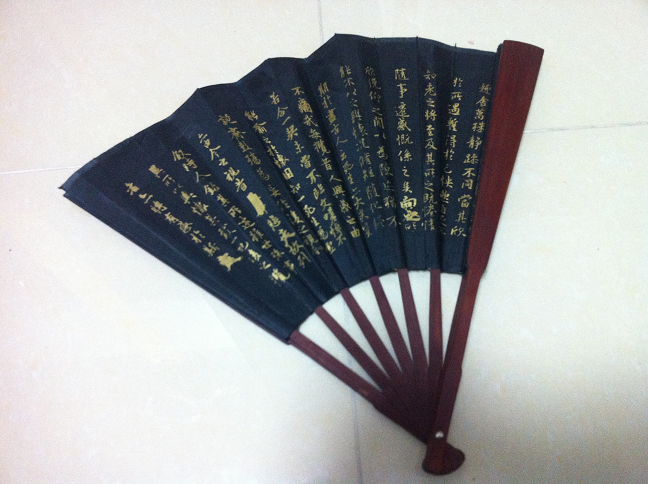
\includegraphics[scale=0.3]{img/fold-fan2.eps}} 
    \subfloat[The fan is fully folded, closed to a stick.]{
\includegraphics[scale=0.3]{img/fold-fan3.eps}}
    \caption{Folding a Chinese hand-fan} \label{fig:fold-fan}
\end{figure}

We can considered that each bamboo frame along with the paper on it as an element, so these frames forms a
list. A unit process to close the fan is to rotate a frame for a certain angle, so that it lays on top
of the collapsed part. When we start close the fan, the initial collapsed result is the first bamboo frame.
The close process is folding from one end, and repeatedly apply the unit close steps, till all the frames
is rotated, and the folding result is a stick closed form.

Actually, the sum and product algorithm exactly do the same thing as close the fan.

\[
\begin{array}{rl}
sum(\{1, 2, 3, 4, 5 \}) & = 1 + (2 + (3 + (4 + 5))) \\
         & = 1 + (2 + (3 + 9)) \\
         & = 1 + (2 + 12) \\
         & = 1 + 14 \\
         & = 15
\end{array}
\]

\[
\begin{array}{rl}
product(\{1, 2, 3, 4, 5 \}) & = 1 \times (2 \times (3 \times (4 \times 5))) \\
         & = 1 \times (2 \times (3 \times 20)) \\
         & = 1 \times (2 \times 60) \\
         & = 1 \times 120 \\
         & = 120
\end{array}
\]

In functional programming, we name this process {\em folding}, and particularly, since we execute from
the most inner structure, which starts from the right-most one. This type of folding is named 
{\em folding right}.

\be
foldr(f, z, L) = \left \{
  \begin{array}
  {r@{\quad:\quad}l}
  z & L = \Phi \\
  f(l_1, foldr(f, z, L')) & otherwise
  \end{array}
\right.
\ee

Let's see how to use fold-right to realize sum and product.

\be
\begin{array}{rl}
\sum_{i=1}^{N} x_i & = x_1 + (x_2 + (x_3 + ... + (x_{N_1} + x_{N}))...) \\
             & = foldr(+, 0, \{x_1, x_2, ..., x_N\})
\end{array}
\ee

\be
\begin{array}{rl}
\prod_{i=1}^{N} x_i & = x_1 \times (x_2 \times (x_3 \times ... + (x_{N_1} \times x_{N}))...) \\
         & = foldr(\times, 0, \{x_1, x_2, ..., x_N\})
\end{array}
\ee

The insertion-sort algorithm can also be defined by using folding right.

\be
sort(L) = foldr(insert, \Phi, L)
\ee

\subsection{folding from left}

As mentioned in section of `tail recursive` call. Both pure recursive sum and product compute from right
to left and they must book keep all the intermediate results and context. As we abstract fold-right from
the very same structure, folding from right does the book keeping as well. This will be expensive if
the list is very long.

Since we can change the realization of sum and product to tail-recursive call manner, it quite possible
that we can provide another folding algorith, which processes the list from left to right in normal order,
and enable the tail-call optimization by reusing the same context.

Instead of induction from sum, product and insertion, we can directly change the folding right to tail call.
Observe that the initial value $z$, actually represents the intermediate result at any time. We can use it
as the accumulator.

\be
foldl(f, z, L) = \left \{
  \begin{array}
  {r@{\quad:\quad}l}
  z & L = \Phi \\
  foldl(f, f(z, l_1), L') & otherwise
  \end{array}
\right.
\ee

Every time when the list isn't empty, we take the first element, apply function $f$ on the accumulator
$z$ and it to get a new accumulator $z' = f(z, l_1)$. After that we can repeatedly folding with the very
same function $f$, the updated accumulator $z'$, and list $L'$.

Let's verify that this tail-call algorithm actually folding from left. 

\[
\begin{array}{rl}
\sum_{i=1}^{5}i & = foldl(+, 0, \{1, 2, 3, 4, 5\}) \\
                & = foldl(+, 0 + 1, \{ 2, 3, 4, 5 \}) \\
                & = foldl(+, (0 + 1) + 2 \{3, 4, 5 \} \\
                & = foldl(+, ((0 + 1) + 2) + 3, \{4, 5\}) \\
                & = foldl(+, (((0 + 1) + 2) + 3) + 4, \{5\}) \\
                & = foldl(+, ((((0 + 1) + 2 + 3) + 4 + 5, \Phi) \\
                & = 0 + 1 + 2 + 3 + 4 + 5
\end{array}
\]

Note that, we actually delayed the evaluation of $f(z, l_1)$ in every step. (This is the exact behavior
in system support lazy-evaluation, for instance, Haskell.) Actually, they will be evaluated in sequence
of $\{ 1, 3, 6, 10, 15\}$ in each call.

Generally, folding-left can be expanded in form of

\be
foldl(f, z, L) = f(f(...(f(f(z, l_1), l_2), ..., l_N)
\ee

Or in infix manner as

\be
foldl(f, z, L) = ((...(z \oplus_f l_1) \oplus_f l_2) \oplus_f ...) \oplus l_N
\ee

With folding from left defined, sum, product, and insertion-sort can be transparently implemented by calling
$foldl$ as $sum(L) = foldl(+, 0, L)$, $product(L) = foldl(+, 1, L)$, and $sort(L) = foldl(insert, \Phi, L)$.
Compare with the folding-right version, they are almost same at first glarence, however, the internal implementation
differs.

\subsubsection{Imperative folding and generic folding concept}
The tail-call nature of folding-left algorithm is quite friendly for imperative settings, that even the compiler
don't equipped with tail-call recursive optimization, we can anyway implement the folding in while-loop manually.

\begin{algorithmic}
\Function{Fold}{$f, z, L$}
  \While{$L \neq Phi$}
    \State $z \gets f(z, $ \Call{First}{$L$} $)$
    \State $L \gets$ \Call{Rest}{$L$}
  \EndWhile
  \State \Return $z$
\EndFunction
\end{algorithmic}

Translating this algorithm to Python yields the following example program.

\lstset{language=Python}
\begin{lstlisting}
def fold(f, z, xs):
    for x in xs:
        z = f(z, x)
    return z
\end{lstlisting}

Actually, Python provide built-in function `reduce' which does the very same thing. (in ISO C++, this is
provided as reduce algorithm in STL.) Almost no imperative environment provides folding-right function because
it will cause stack overflow problem if the list is too long. However, in case the folding from right
semantics is neccessary, For example, one defines a container, which only provides insertion function to
the head of the container, but there is no any appending method, so that we want such a $fromList$
tool.

\[
fromList(L) = foldr(insertHead, empty, L)
\]

Calling $fromList$ with the insertion function as well as an empty intialized container, can turn a list 
into the special container. Actually the singly linked-list is such a container, which performs well
on insertion to the head, but poor to linear time if appending on the tail. Folding from right is quite
nature when duplicate a linked-list while keeps the elements order. While folding from left will generates
a reversed list.

In such case, there exists an alternative way to implement imperative folding right by first reverse the list, and then
folding the reversed one from left.

\begin{algorithmic}
\Function{Fold-Right}{$f, z, L$}
  \State \Return \textproc{Fold}($f, z$, \Call{Reverse}{$L$})
\EndFunction
\end{algorithmic}

Note that, here we must use the tail-call version of reversing, or the stack overflow issue still exists.

One may think that folding-left should be chosen in most cases over folding-right because it's friendly for 
tail-recursion call optimization, suitable for both functional and imperative settings, and it's online
algorithm. However, folding-right plays a critical role when the input list is infinity and the binary function
$f$ is lazy. For example, below Haskell program wrap every element of an infinity list to a singleton, and
returns the first 10 result.

\lstset{language=Haskell}
\begin{lstlisting}
take 10 $ foldr (\x xs ->[x]:xs) [] [1..]
[[1], [2], [3], [4], [5], [6], [7], [8], [9], [10]]
\end{lstlisting} %$

This can't be achieved by using folding left because the outter most evaluation can't be finished untill
all the list being processed. The details is specific to lazy evaluation feature, which is out of the 
scope of this book. Readers can refer to \cite{Haskell-wiki} for details.

Althought the main topic of this appendix is about single linked-list related algorithms, the folding
concept itself is generic which doesn't only limit to list, but also can be applied to other data structures.

We can fold a tree, a queue, or even more complicated data structures as long as we have the following:

\begin{itemize}
\item The empty data structure can be identified for trivial edge case; (e.g. empty tree)
\item We can traverse the data structure (e.g. pre-order travres the tree).
\end{itemize}

Some languages provide this high-level concept support, for example, Haskell achieve this via
{\em monoid}, readers can refer to \cite{learn-haskell} for detail.

There are many chapters in this book use the widen concept of folding.

\subsection{folding in practice}

We have seen that $max$, $min$, and insertion sort all can be realized in folding. The 
brute-force solution for `drunk jailer' puzzle shown in mapping section can also be
designed by mixed use of mapping and folding.

Remind that we create a list of pairs, each pair contains the number of the light, and 
the on-off state. After that we process from 1 to $N$, switch the light if the number
can be divided. The whole process can be viewed as folding.

\[
fold(step, \{(1, 0), (2, 0), ..., (N, 0) \}, \{1, 2, ..., N\})
\]

The initial value is the very first states, that all the lights are off. The list to be
foding is the operations from 1 to $N$. Function $step$ takes two arguments, one is
the light states pair list, the other is the operation time $i$. It then maps
on all lights and performs switching. We can then subtitute the $step$ with mapping.

\[
fold(\lambda_{L, i} map(switch(i), L), \{(1, 0), (2, 0), ..., (N, 0) \}, \{1, 2, ..., N\})
\]

We'll simplify the $\lambda$ notation, and directly write $map(switch(i), l)$ for brevity purpose.
The result of this folding is the final states pairs, we need take the second one of the pair
for each element via mapping, then calculate the summation.

\be
sum(map(snd, fold(map(switch(i), L), \{(1, 0), (2, 0), ..., (N, 0) \}, \{1, 2, ..., N\})))
\ee

There are materials provides plenty of good examples of using folding, especially in \cite{fp-pearls},
folding together with fusion law are well explained.

\subsubsection{concatenate a list of list}

In previous section \ref{concat} about concatenation, we explained how to concatenate two lists.
Actually, concatenation of lists can be considered equivallent to summation of numbers. Thus we
can design a general algorithm, which can concatenate mutliple lists into one big list.

What's more, we can realize this general concatenation by using folding. As sum can be represented
as $sum(L) = foldr(+, 0, L)$, it's straightforward to write the following equation.

\be
concats(L) = foldr(concat, \Phi, L)
\ee

Where $L$ is a list of list, for example $\{\{1, 2, 3\}, \{4, 5, 6\}, \{7, 8, 9\}, ...\}$. Function 
$concat(L_1, L_2)$ is what we defined in section \ref{concat}.

In some environment which supports lazy-evaluation, such as Haskell, this algorithm is capable to 
concatenate infinite list of list, as the binary function \verb|++| is lazy, and the folding-right
is actually tail-call.

\section{Searching and matching}

Searching and matching is one type of the most important algorithms not only limits to linked list.
We just scratch the surface of it in this appendix. There are dedicated chapters explain about them.

\subsection{Existence testing}

The simplest searching case is to test if a given element exists in a list, a linear time traverse
can solve this problem. In order to determin element $x$ exists in elements $L$.

\begin{itemize}
\item If the list is empty, it obvious that the element doesn't exist in $L$;
\item If the first element in the list equals to $x$, we know that $x$ exists;
\item Otherwise, we need recursively test if $x$ exists in the rest sub-list $L'$;
\end{itemize}

This simple description can be directly formalized to equations as the following.

\be
x \in L =  \left \{
  \begin{array}
  {r@{\quad:\quad}l}
  False & L = \Phi \\
  True & l_1 = x \\
  x \in L' & otherwise
  \end{array}
\right.
\ee

This is definitely linear algorithm which is bound to $O(N)$ time. The best case
happens in the two trivial cases that either the list is empty or the first element
is what we are finding; The worst case happens when the elements doesn't exist at all
or it is the last element, in both case, we need traverse the whole list. If the probability
is equal for all the position, the average case takes about $\frac{N+1}{2}$ steps 
for traversing.

This algorithm is so trivial that we left the implementation as exercise to the reader.
If the list is orderred, one may expect to improve the algorithm to logarithm time
but not linear. However, as we dicussed, since list doesn't support constant time
random accessing, binary search can't be applied here. There is a dedicated chapter
in this book discusses how to evolute the linked list to binary tree to achieve
quick searching.

\subsection{Looking up}

One extra step from existence testing is to find the intersting information stored in the list.
There are two typical methods to augment extra data to the element. Since the linked list is chain
of nodes, we can store sitellite data in the node, then provide $key(n)$ to access the
key of the node, $rest(n)$ for the rest sub-list, and $value(n)$ for the augmented data.
The other method, is to pair the key and data, for example $\{(1, hello), (2, world), (3, foo), ...\}$.
We'll introduce how to form such pairing list in later section.

The algorithm is almost as same as the existence testing, that it traverses the list, examines
the key one by one. Whenever it finds a node which has the same key as what we are looking up,
it stops, and returns the augmented data. It's obvious that this is linear strategy.
If the sitelite data is augmented to the node directly,
the algorithm can be defined as the following.

\be
lookup(x, L) = \left \{
  \begin{array}
  {r@{\quad:\quad}l}
  \Phi & L = \Phi \\
  value(l_1) & key(l_1) = x \\
  lookup(x, L') & otherwise
  \end{array}
\right.
\ee

In this algorithm, $L$ is a list of nodes which are augmented with sitelite data. Note that
the first case actually means looking up failure, so that the result is empty. Some functional 
programming languages, such as Haskell, provide \verb|Maybe| type to handle the possibility of
fail. This algorithm can be slightly modified to handle the key-value pair list.

\be
lookup(x, L) = \left \{
  \begin{array}
  {r@{\quad:\quad}l}
  \Phi & L = \Phi \\
  snd(l_1) & fst(l_1) = x \\
  lookup(x, L') & otherwise
  \end{array}
\right.
\ee

Here $L$ is a list of pairs, functions $fst(p)$ and $snd(p)$ access the first part and second part
of the pair respectively.

Both algorithms are in tail-call manner, they can be transform to imperative looping easily. We
left this as exercise to the reader.

\subsection{finding and filtering}

Let's take one more step ahead, looking up algorithm performs linear search by comparing the
key of an element is equal to the given value. A more general case is to find an element match
a certain predicate. We can abstract this matching condition as a parameter for this generic
linear finding.

\be
find(p, L) =  \left \{
  \begin{array}
  {r@{\quad:\quad}l}
  \Phi & L = \Phi \\
  l_1 & p(l_1) \\
  find(p, L') & otherwise
  \end{array}
\right.
\ee

The algorithm traverses the list by examine if the element satisfies the predicate $p$. It
fails if the list is empty while there is still nothing found. This is handled in the first
trivial edge case; If the first element in the list satisfies the condition, the algorithm
returns the whole element (node), and user can further handle it as he like (either extract 
the sitelite data or do whatever); otherwise, the algorithm recursively perform finding
on the rest of the sub-list. Below is the corresponding Haskell example program. 

\lstset{language=Haskell}
\begin{lstlisting}
find _ [] = Nothing
find p (x:xs) = if p x then Just x else find p xs
\end{lstlisting}

Translating this to imperative algorithm is straightforward. Here we use 'NIL' to represent
the fail case.

\begin{algorithmic}
\Function{Find}{$p, L$}
  \While{$L \neq \Phi$}
    \If{$p$(\Call{First}{$L$})}
      \State \Return \Call{First}{$L$}
    \EndIf
    \State $L \gets$ \Call{Rest}{$L$}
  \EndWhile
  \State \Return NIL
\EndFunction
\end{algorithmic}

And here is the Python example of finding.

\lstset{language=Python}
\begin{lstlisting}
def find(p, xs):
    for x in xs:
        if p(x):
            return x
    return None      
\end{lstlisting}

It's quite possible that there are multiple elements in the list which satisfiy the precondition.
The finding algorithm designed so far just pick the first one it meets and stops immediately.
It can be considered as a special case of finding all elements under a certain condition.

Another viewpoint of finding all elements with a given predicate is treat the finding algorithm
as a black box, the input to this box is a list, while the output is another list contains
all elements satisfy the predicate. This can be called as filtering as shown in the below
figure.

\begin{figure}[htbp]
        \centering
        \includegraphics[scale=0.8]{img/filter.ps}
        \caption{The input is the original list $\{x_1, x_2, ..., x_N\}$, the output is a list $\{x_1', x_2', ..., x_M'\}$, that for $\forall x_i'$, predicate $p(x_i')$ is satisified.} \label{fig:filter}
\end{figure}

This figure can be formalized in another form in tast of set enumeration. However, we actually
enumerate among list instead of a set.

\be
filter(p, L) = \{ x | x \in L \land p(x) \}
\ee

Some environment such as Haskell (and Python for any iterable), supports this form as list comprehension.

\lstset{language=Haskell}
\begin{lstlisting}
filter p xs = [ x | x <- xs, p x]
\end{lstlisting}

And in Python for built-in list as

\lstset{language=Python}
\begin{lstlisting}
def filter(p, xs):
    return [x for x in xs if p(x)]
\end{lstlisting}

Note that the Python built-in list isn't singly-linked list as we mentioned in this appendix.

In order to modify the finding algorithm to realize the filtering, the found element is appended
to a result list. And instead of stop the traverse, all the rest of elements should be examined
with the predicate.

\be
filter(p, L) = \left \{
  \begin{array}
  {r@{\quad:\quad}l}
  \Phi & L = \Phi \\
  cons(l_1, filter(p, L')) & p(l_1) \\
  filter(p, L') & otherwise
  \end{array}
\right.
\ee

This algorithm returns empty result if the list is empty for trivial edge case; For non-empty list,
suppose the recursive result of filtering the rest of the sub-list is $A$, the algorithm examine
if the first element satisfy the predicate, it is put in front of $A$ by a `cons' operation ($O(1)$ time).

The corresponding Haskell program is given as below.

\lstset{language=Haskell}
\begin{lstlisting}
filter _ [] = []
filter p (x:xs) = if p x then x : filter p xs else filter p xs
\end{lstlisting} 

Although we mentioned that the next found element is `appended' to the result list, this algorithm
actually constructs the result list from the right most to the left, so that appending 
is avoided, which ensure the linear $O(N)$ performance. Compare this algorithm with the following
imperative quadratic realization reveals the difference.

\begin{algorithmic}
\Function{Filter}{$p, L$}
  \State $L' \gets \Phi$
  \While{$L \neq \Phi$}
    \If{$p$(\Call{First}{$L$})}
      \State $L' \gets$ \textproc{Append}($L'$, \Call{First}{$L$}) \Comment{Linear operation}
    \EndIf
    \State $L \gets$ \Call{Rest}{$L$}
  \EndWhile
\EndFunction
\end{algorithmic}

As the comment of appending statement, it's typically proportion to the length of the result list
if the tail position isn't memorized. This fact indicates that directly transforming the recursive filter
algorithm into tail-call form will downgrade the performance from $O(N)$ to $O(N^2)$. As shown
in the below equation, that $filter(p, L) = filter'(p, L, \Phi)$ performs as poorly as the 
imperative one.

\be
filter'(p, L, A) = \left \{
  \begin{array}
  {r@{\quad:\quad}l}
  A & L = \Phi \\
  filter'(p, L', A \cup \{l_1\}) & p(l_1) \\
  filter'(p, L', A) & otherwise
  \end{array}
\right.
\ee

One solution to achieve linear time performance imperatively is to construct the result list in
reverse order, and perform the $O(N)$ reversion (refer to the above section) to get the final result.
This is left as exercise to the reader.

The fact of construction the result list from right to left indicates the possibility of realizing
filtering with folding-right concept. We need design some combinator function $f$, so that
$filter(p, L) = foldr(f, \Phi, L)$. It requires that function $f$ takes two arguments, one 
is the element iterated among the list; the other is the intermediate result constructed 
from right. $f(x, A)$ can be defined as that it tests the predicate against $x$, if succeed,
the result is updated to $cons(x, A)$, otherwise, $A$ is kept same.

\be
f(x, A) = \left \{
  \begin{array}
  {r@{\quad:\quad}l}
  cons(x, A) & p(x) \\
  A & otherwise
  \end{array}
\right.
\ee

However, the predicate must be passed to function $f$ as well. This can be achieved by using
curring, so $f$ actually has the prototype $f(p, x, A)$, and filtering is defined as follow.

\be
filter(p, L) = foldr(\lambda_{x, A} \cdot f(p, x, A), \Phi, L)
\ee

Which can be simplified by $\eta$-convertion. For detailed definition of $\eta$-convertion,
readers can refer to \cite{slpj-book-1987}.

\be
filter(p, L) = foldr(f(p), \Phi, L)
\ee

The following Haskell example program imlements this equation.

\lstset{language=Haskell}
\begin{lstlisting}
filter p = foldr f [] where
    f x xs = if p x then x : xs else xs
\end{lstlisting}

Similar like mapping and folding, filtering is actually a generic concept, that we can apply
a predicate on any traversable data structures to get what we are interesting. readers can 
refer to the topic about monoid in \cite{learn-haskell} for further reading.

\subsection{Matching}

Matching generally means to find a given parttern among some data structures. In this section,
we limit the topic within list. Even this limitation will leads to a very wide and deep topic,
that there are dedicated chapters in this book introduce matching algorithms. So we only select
the algorithm to test if a given list exists in another (typically longer) list.

Before dive into the algorithm of finding the sub-list at any position, two special edge cases
are used for warm up. They are algorithms to test if a given list is either prefix or postfix 
of another.

In the section about span, we have seen how to find a prefix under a certain condition.
prefix matching can be considered as a special case in some sense. That it compares each
of the elements between the two from the beginning until meets any different elements
or pass the end of one list. Define $P \subseteq L$ if $P$ is prefix of $L$.

\be
P \subseteq L = \left \{
  \begin{array}
  {r@{\quad:\quad}l}
  True & P = \Phi \\
  False & p_1 \neq l_1 \\
  P' \subseteq L' & otherwise
  \end{array}
\right.
\ee

This is obviously a linear algorithm. However, We can't use the very same approach 
to test if a list is postfix of another because it isn't cheap to start from the
end of the list and keep iterating backward. Arrays, on the other hand which support
random access can be easily traversed backward.

As we only need the yes-no result, one solution to realize a linear postfix testing
algorithm is to reverse both lists, (which is linear time), and use prefix testing
instead. Defind $L \supseteq P$ if $P$ is postfix of $L$.

\be
L \supseteq P = reverse(P) \subseteq reverse(L)
\ee

With $\subseteq$ defined, it enables to test if a list is infix of another.
The idea is to traverse the target list, and repeatedly applying the prefix testing
till any success or arrives at the end.

\begin{algorithmic}
\Function{Is-Infix}{$P, L$}
  \While{$L \neq \Phi$}
    \If{$P \subseteq L$}
      \State \Return TRUE
    \EndIf
    \State $L \gets$ \Call{Rest}{$L$}
  \EndWhile
  \State \Return FALSE
\EndFunction
\end{algorithmic}

Formalize this algorithm to recursive equation leads to the below definition.

\be
infix?(P, L) = \left \{
  \begin{array}
  {r@{\quad:\quad}l}
  True & P \subseteq L \\
  False & L = \Phi \\
  infix?(P, L') & otherwise
  \end{array}
\right.
\ee

Note that there is a tricky implicit constraint in this equation. If the pattern $P$ is empty,
it is definitely the infix of any target list. This case is actually covered by the first condition
in the above equation becasue empty list is also the prefix of any list. In most programming languages
support pattern matching, we can't arrange the second clause as the first edge case, or it will
return false for $infix?(\Phi, \Phi)$. (One exception is Prolog, but this is language spcific 
feature, which we won't covered in this book.)

Since prefix testing is linear, and it is called while traverse the list, this algorithm 
is quadratic $O(N*M)$. where $N$ and $M$ are the length of the pattern and target lists respectively.
There is no trivial way to improve this position by position scanning algorithm to linear
even if the data strucutre changes from linked-list to randomly accessible array.

There are chapters in this book introduce several approaches for fast matching, including 
suffix tree with Ukkonen algorithm, Knuth-Morris-Pratt algorithm and Boyer-Moore algorithm.

Alternatively, we can enumerate all suffixes of the target list, and check if the pattern 
is prefix of any these suffixes. Which can be represented as the following.

\be
infix?(P, L) = \exists S \in suffixes(L) \land P \subseteq S
\ee

This can be represented as list enumeration, for example the below Haskell program.

\lstset{language=Haskell}
\begin{lstlisting}
isInfixOf x y = (not . null) [ s | s <- tails(y), x `isPrefixOf`s]
\end{lstlisting}

Where function \verb|isPrefixOf| is the prefixing testing function defined according to
our previous design. function \verb|tails| generate all suffixes of a list. The implementation
of \verb|tails| is left as an exercise to the reader.

\begin{Exercise}
\begin{itemize}
\item Implement the linear existence testing in both functional and imperative approaches in 
your favorite programming languages.
\item Implement the looking up algorithm in your favorite imperative programming language.
\item Realize the linear time filtering algorith by firstly building the result list in reverse
order, and finally reverse it to resume the normal result. Implement this algorith in both
imperative looping and functional tail-recursion call.
\item Implement the imperative algorithm of prefix testing in your favorite programming language.
\item Implmeent the algorithm to enumerate all suffixes of a list.
\end{itemize}
\end{Exercise}

\section{zipping and unzipping}

It's quite commonly to construct a list of paired elements, for example, in the naive 
brute-force solution for 'Drunk jailer' puzzle which is shown in section of mapping,
we need to represents the states of each lights. It is initialized as $\{(1, 0), (2, 0), ..., (N, 0)\}$.
Another example is to build a key-value list, such as $\{(1, a), (2, an), (3, another), ... \}$.

In 'Drunk jailer' example, the list of pairs is built like the following.

\[
map(\lambda_i \cdot (i, 0), \{1, 2, ..., N\})
\]

The more general case is taht, There have been already two lists prepared, what we need
is a handy `zipper' method.

\be
zip(A, B) = \left \{
  \begin{array}
  {r@{\quad:\quad}l}
  \Phi & A = \Phi \lor B = \Phi \\
  cons((a_1, b_1), zip(A', B')) & otherwise
  \end{array}
\right.
\ee

Note that this algorithm is capable to handle the case that the two lists being zipped have different
lengths. The result list of pairs alignes with the shorter one. And it's even posssible to zip
an infinit list with another one with limited length. For example with this auxiliary function defined, 
we can initialize the lights state as 

\[
zip(\{0, 0, ...\}, \{1, 2, ..., N\}
\]

In some language supports list enumeration, such as Haskell (Python provides similiar \verb|range| function, but it
manipulates built-in list, which isn't linked-list actually), this can be expressed as \verb|zip (repeat 0) [1..n]|.
Given a list of words, we can also index them with consequtive numbers as 

\[
zip(\{1, 2, ...\}, \{a, an, another, ...\})
\]

Note that the zipping algorithm is linear, as it uses constant time `cons' operation in each recursive call.
However, directly translating $zip$ into imperative manner would down-grade the performance to quadratic 
unless the linked-list is optimized with tail position cache or we in-place modify one of the passed-in list.

\begin{algorithmic}
\Function{Zip}{$A, B$}
  \State $C \gets \Phi$
  \While{$A \neq \Phi \land B \neq \Phi$}
    \State $C \gets $ \textproc{Append}(C, (\Call{First}{$A$}, \Call{First}{$B$}))
    \State $A \gets$ \Call{Rest}{$A$}
    \State $B \gets$ \Call{Rest}{$B}$
  \EndWhile
  \State \Return $C$
\EndFunction
\end{algorithmic}

Note that, the appending operation is proportion to the length of the result list $C$, so it will get
more and more slowly along with traversing. There are three solutions to improve this algorithm to
linear time. The first method is to use a similar approach as we did in infix-testing, that we construct
the result list of pairs in reverse order by always insert the paired elements on head; then perform
a linear reverse operation before return the final result; The second method is to modify one passed-in
list, for example $A$, in-place while traversing. Translate it from list of elemnts to list of pairs;
The third method is remembered the last appending position. Please try these solutions as exercise.

The key point of linear time zipping is that the result list is actually built from right to left, which
is similiar to the infix-testing algorithm. So it's quite possible to provide a folding-right realization.
This is left as exercise to the reader.

It's natural to extend the zipper algorithm so that multiple lists can be zipped to one list of multip-elements.
For example, Haskell standard library provides, \verb|zip|, \verb|zip3|, \verb|zip4|, ..., till \verb|zip7|.
Another typicall extension to zipper is that, some times, we don't want to list of pairs (or tuples
more generally), instead, we want to apply some combinator function to each pair of elements.

For example, consider the case that we have a list of unit prices for every fruit apple, orange, banana, ...,
 as $\{1.00, 0.80, 10.05, ...\}$, with same unit of Dollar; And the cart of customer holds a list
of purchased quantity, for instance $\{3, 1, 0, ...\}$, means this customer, put 3 apples, an orange in the
cart. He doesn't take any banana, so tht quantity is zero. We want to generate a list of cost for the 
customer, contains how much should pay for apple, orange, banana,... respectively.

The program can be written from scratch as below.

\[
paylist(U, Q) =  \left \{
  \begin{array}
  {r@{\quad:\quad}l}
  \Phi & U = \Phi \lor Q = \Phi \\
  cons(u_1 \times q_1, paylist(U', Q')) & otherwise
  \end{array}
\right.
\]

Compare this equation with the zipper algorithm. It's easy to find the common structure of the two, and
we can parameterize the combinator function as $f$, so that the `generic' zipper algorithm can be
defined as the following.

\be
zipWith(f, A, B) = \left \{
  \begin{array}
  {r@{\quad:\quad}l}
  \Phi & A = \Phi \lor B = \Phi \\
  cons(f(a_1, b_1), zipWith(f, A', B')) & otherwise
  \end{array}
\right.
\ee

Here is an example that defines the inner-product (or dot-product)\cite{wiki-dot-product} by using $zipWith$.

\be
A \cdot B = sum(zipWith(\times, A, B))
\ee

TODO: unzip
TODO: General zipper and unzipper concept.

\begin{Exercise}
\begin{itemize}
\item Design and implments iota ($I$) algorithm, which can enumerate a list with some given parameters. For example:
  \begin{itemize}
  \item $iota(..., N) = \{1, 2, 3, ..., N\}$;
  \item $iota(M, N) = \{M, M+1, M+2, ..., N\}$, Where $M \leq N$;
  \item $iota(M, M+a, ..., N) = \{M, M+a, M+2a, ..., N \}$;
  \item $iota(M, M, ...) = repeat(M) = \{M, M, M, ...\}$;
  \item $iota(M, ...) = \{M, M+1, M+2, ... \}$.
  \end{itemize}
  Note that the last two cases demands generate infinit list essentially. Consider how to represents infinit list?
  You may refer to the streaming and lazy evaluation materials such as \cite{SICP} and \cite{learn-haskell}.
\item Design and implement a linear time imperative zipper algorithm.
\item Realize the zipper algorithm with folding-right approach.
\end{itemize}
\end{Exercise}

% ================================================================
%                 Short summary
% ================================================================
\section{Notes and short summary}
...

% ================================================================
%                 Appendix
% ================================================================

\begin{thebibliography}{99}

\bibitem{fp-pearls}
Richard Bird. ``Pearls of Functional Algorithm Design''. Cambridge University Press; 1 edition (November 1, 2010). ISBN: 978-0521513388

\bibitem{slpj-book-1987}
Simon L. Peyton Jones. ``The Implementation of Functional Programming Languages''. Prentice-Hall International Series in Computer Since. Prentice Hall (May 1987). ISBN: 978-0134533339

\bibitem{moderncxx}
Andrei Alexandrescu. ``Modern C++ design: Generic Programming and Design Patterns Applied''. Addison Wesley February 01, 2001, ISBN 0-201-70431-5

\bibitem{mittype}
Benjamin C. Pierce. ``Types and Programming Languages''. The MIT Press, 2002. ISBN:0262162091

\bibitem{SICP}
Harold Abelson, Gerald Jay Sussman, Julie Sussman. ``Structure and Interpretation of Computer Programs, 2nd Edition''. MIT Press, 1996, ISBN 0-262-51087-1

\bibitem{okasaki-book}
Chris Okasaki. ``Purely Functional Data Structures''. Cambridge university press, (July 1, 1999), ISBN-13: 978-0521663502

\bibitem{learn-haskell}
Miran Lipovaca. ``Learn You a Haskell for Great Good! A Beginner's Guide''. No Starch Press; 1 edition April 2011, 400 pp. ISBN: 978-1-59327-283-8

\bibitem{wiki-tail-call}
Wikipedia. ``Tail call''. https://en.wikipedia.org/wiki/Tail\_call

\bibitem{sgi-stl-transform}
SGI. ``transform''. http://www.sgi.com/tech/stl/transform.html

\bibitem{poj-drunk-jailer}
ACM/ICPC. ``The drunk jailer.'' Peking University judge online for ACM/ICPC. http://poj.org/problem?id=1218.

\bibitem{Haskell-wiki}
Haskell wiki. ``Haskell programming tips''. 4.4 Choose the appropriate fold. http://www.haskell.org/haskellwiki/Haskell\_programming\_tips

\bibitem{wiki-dot-product}
Wikipedia. ``Dot product''. http://en.wikipedia.org/wiki/Dot\_product

\end{thebibliography}

\ifx\wholebook\relax \else
\end{document}
\fi

% LocalWords:  typedef struct typename
